% 中文译文；章标题由主文件提供，覆盖范围见 coverage/XX.json。
\markboth{第 XX 讲. 半单秩为 1 的约化群}{第 XX 讲. 半单秩为 1 的约化群}
\SGARefTarget{sga3:xx:expose}
\setcounter{footnote}{0}
\footnotetext{编者注: 2024 年 10 月 13 日版本.}

\section{初等系. 群 \texorpdfstring{\(U_\alpha\)}{Uα} 与 \texorpdfstring{\(U_{-\alpha}\)}{U−α}}
\SGARefTarget{sga3:xx:section:1}
\paragraph{\textbf{回顾 \SGARefLink{sga3:xx:section:1}{1.1}.}}
\SGARefTarget{sga3:xx:1.1}
\emph{设 \(S=\Spec(k)\), 其中 \(k\) 为代数闭域; 设 \(G\) 为半单秩为一的约化 \(S\)-群, \(T\) 为 \(G\) 的极大环面, 它必分裂. 则}
\[
  \mathfrak g=\mathfrak t\oplus\mathfrak g^\alpha
  \oplus\mathfrak g^{-\alpha},
\]
\emph{其中 \(\alpha\) 和 \(-\alpha\) 是 \(G\) 关于 \(T\) 的根. 此外存在两个群单态射}
\[
  p_\alpha\colon\mathbb G_{a,S}\longrightarrow G,
  \qquad
  p_{-\alpha}\colon\mathbb G_{a,S}\longrightarrow G
\]
\emph{使对每个 \(S'\to S\)、\(t\in T(S')\) 及 \(x\in\mathbb G_a(S')\), 都有}
\[
  t\,p_\alpha(x)\,t^{-1}=p_\alpha\bigl(\alpha(t)x\bigr),
  \qquad
  t\,p_{-\alpha}(x)\,t^{-1}
    =p_{-\alpha}\bigl(\alpha(t)^{-1}x\bigr)
\]
\emph{并且态射}
\[
  \mathbb G_{a,S}\times_S T\times_S\mathbb G_{a,S}
    \longrightarrow G,
  \qquad
  (y,t,x)\longmapsto p_{-\alpha}(y)\,t\,p_\alpha(x),
\]
\emph{是根式态射 (radicial) 且占优 \textup{(\emph{Bible}, §13.4, 定理 3 的推论 2)}.}

由于这一态射在单位元处的切映射是双射, 它也是可分的, 因而是双有理的. 由 Zariski 主定理 \textup{(EGA III\(_1\), 4.4.9)}, 它是开浸入.

\paragraph{\textbf{引理 1.2.}}
\SGARefTarget{sga3:xx:1.2}
\emph{设 \(S\) 是概形, \(G\) 是 \(S\)-群概形, \(T\) 是 \(G\) 的环面, \(Q\) 是 \(T\) 的子环面, \(\alpha\) 是 \(T\) 的一个特征, 其在 \(Q\) 上的限制在每个纤维上均非平凡. 设
\[
  p_\alpha\colon\mathbb G_{a,S}\longrightarrow G
  \quad\textup{和}\quad
  p_{-\alpha}\colon\mathbb G_{a,S}\longrightarrow G
\]
是分别被 \(T\) 以乘子 \(\alpha\) 及 \(-\alpha\) 正规化的群态射. 假设态射
\[
  u\colon\mathbb G_{a,S}\times_S T\times_S\mathbb G_{a,S}
    \longrightarrow G,
  \qquad
  u(y,t,x)=p_{-\alpha}(y)\,t\,p_\alpha(x),
\]
在点上由所示公式定义, 是开浸入. 最后, 设 \(q\geq 0\) 是整数,
\[
  p\colon\mathbb G_{a,S}\longrightarrow G
\]
是群态射, 使对每个 \(S'\to S\)、\(t\in Q(S')\) 及 \(x\in\mathbb G_a(S')\), 都有
\[
  \intaut(t)^q\bigl(p(x)\bigr)=p\bigl(\alpha(t)x\bigr).
\]
则存在唯一的 \(\nu\in\mathbb G_a(S)\), 使
\[
  p(x)=p_\alpha(\nu x^q).
\]}

事实上, 设 \(\Omega\) 是 \(u\) 的像, 令 \(U=p^{-1}(\Omega)\). 这是 \(\mathbb G_{a,S}\) 的一个包含零截面的开子集. 对 \(Q\) 的每个截面 \(t\), 乘以 \(\alpha(t)\) 使 \(U\) 整体不变. 有 \(U=\mathbb G_{a,S}\). 只须在 \(S\) 为代数闭域 \(k\) 的谱时验证; 此时
\[
  \alpha\colon Q(k)\longrightarrow k^\times
\]
为满射, 所以 \(U(k)\supset k^\times\), 从而 \(U=\mathbb G_{a,k}\).

因而存在三个态射
\[
  a\colon\mathbb G_{a,S}\longrightarrow\mathbb G_{a,S},
  \qquad
  b\colon\mathbb G_{a,S}\longrightarrow T,
  \qquad
  c\colon\mathbb G_{a,S}\longrightarrow\mathbb G_{a,S}
\]
使
\[
  p(x)=p_{-\alpha}\bigl(a(x)\bigr)\,b(x)\,
       p_\alpha\bigl(c(x)\bigr).
\]
对 \(p\) 的条件成为
\[
  a\bigl(\alpha(t)x\bigr)=\alpha(t)^{-q}a(x),\qquad
  b\bigl(\alpha(t)x\bigr)=b(x),\qquad
  c\bigl(\alpha(t)x\bigr)=\alpha(t)^q c(x).
\]
由同样的理由, 对每个 \(S'\to S\) 及 \(z\in\mathbb G_m(S')\),
\[
  a(zx)=z^{-q}a(x),\qquad b(zx)=b(x),\qquad c(zx)=z^q c(x),
\]
所以
\[
  z^q a(z)=a(1),\qquad b(z)=b(1),\qquad c(z)=z^q c(1).
\]
由于 \(\mathbb G_{m,S}\) 在 \(\mathbb G_{a,S}\) 中概形稠密, 对每个 \(S'\to S\) 及 \(x\in\mathbb G_a(S')\) 得到
\[
\begin{aligned}
  x^q a(x)&=a(1)=a(0)=0, &&\text{故 }a=0,\\
  c(x)&=x^q c(1)=\nu x^q,
    &&\text{其中 }\nu\in\mathbb G_a(S),\\
  b(x)&=b(1)=b(0)=e, &&\text{故 }b=e.
\end{aligned}
\]
证明完成.

\paragraph{\textbf{定义 1.3.}}
\SGARefTarget{sga3:xx:1.3}
\emph{一个 \(S\)-初等系 (elementary system) 是三元组 \((G,T,\alpha)\), 其中}
\begin{enumerate}
\item[\textup{(i)}] \emph{\(G\) 是半单秩为一的约化 \(S\)-群 \textup{(\SGARefLink{sga3:xix:definition:2:7}{第 XIX 讲, 2.7})};}
\item[\textup{(ii)}] \emph{\(T\) 是 \(G\) 的极大环面;}
\item[\textup{(iii)}] \emph{\(\alpha\) 是 \(G\) 关于 \(T\) 的根 \textup{(\SGARefLink{sga3:xix:definition:3-2}{第 XIX 讲, 3.2})}.}
\end{enumerate}
因此有直和分解 \textup{(\SGARefLink{sga3:xix:lemma:3:5}{第 XIX 讲, 3.5})}
\[
  \mathfrak g=\mathfrak t\oplus\mathfrak g^\alpha
  \oplus\mathfrak g^{-\alpha},
\]
其中 \(\mathfrak g^\alpha\) 与 \(\mathfrak g^{-\alpha}\) 都局部自由且秩为一.\footnote{作为 \(\mathcal O_S\)-模而言.}

\paragraph{\textbf{1.4.}}
\SGARefTarget{sga3:xx:1.4}
若 \((G,T,\alpha)\) 为 \(S\)-初等系, 则对每个 \(S'\to S\), \((G_{S'},T_{S'},\alpha_{S'})\) 为 \(S'\)-初等系. 若 \((G,T,\alpha)\) 为 \(S\)-初等系, 则 \((G,T,-\alpha)\) 也是.

若 \(S\) 是概形, \(G\) 是约化 \(S\)-群, \(T\) 是 \(G\) 的极大环面, \(\alpha\) 是 \(G\) 关于 \(T\) 的根, 则 \((Z_\alpha,T,\alpha)\) 为 \(S\)-初等系 \textup{(\SGARefLink{sga3:xix:paragraph:3-9}{第 XIX 讲, 3.9})}.

设 \((G,T,\alpha)\) 为 \(S\)-初等系. 可逆模 \(\mathfrak g^\alpha\) 典范地带有 \(T\)-模结构. 因而向量丛 \(W(\mathfrak g^\alpha)\) 也是 \(T\)-模. 另一方面, \(T\) 的元素的内自同构使 \(G\) 成为一个带算子群 \(T\) 的群.

\paragraph{\textbf{定理 1.5.}}
\SGARefTarget{sga3:xx:1.5}
\emph{设 \((G,T,\alpha)\) 为 \(S\)-初等系.}
\begin{enumerate}
\item[\textup{\SGAInlineRefTarget{sga3:xx:1.5:item:i}(i)}] \emph{存在唯一的带算子群 \(T\) 的群之间的态射
  \[
    \exp\colon W(\mathfrak g^\alpha)\longrightarrow G
  \]
  在 Lie 代数上诱导典范映射 \(\mathfrak g^\alpha\to\mathfrak g\).\footnote{下文\SGARefLink{sga3:xx:5.9}{推论 5.9} 将表明, \(\exp\) 是从 \(W(\mathfrak g^\alpha)\) 到 \(G\) 的一个闭子群的同构.}
  等价地, \(\exp\) 是唯一满足以下条件的态射: 对每个 \(S'\to S\)、\(t\in T(S')\) 及 \(X,X'\in W(\mathfrak g^\alpha)(S')\),
  \[
  \begin{aligned}
    \exp(X+X')&=\exp(X)\exp(X'),\\
    \intaut(t)\bigl(\exp(X)\bigr)&=\exp\bigl(\alpha(t)X\bigr),\\
    \Lie(\exp)(X)&=X.
  \end{aligned}
  \]}
\item[\textup{\SGAInlineRefTarget{sga3:xx:1.5:item:ii}(ii)}] \emph{在 \(S\)-初等系 \((G,T,-\alpha)\) 中类似地定义
  \[
    \exp\colon W(\mathfrak g^{-\alpha})\longrightarrow G.
  \]
  则态射
  \[
    W(\mathfrak g^{-\alpha})\times_S T
      \times_S W(\mathfrak g^\alpha)\longrightarrow G,
    \qquad
    (Y,t,X)\longmapsto \exp(Y)\,t\,\exp(X),
  \]
  在点上由所示公式定义, 是开浸入.}
\end{enumerate}

暂时假设所需的指数态射存在, 来证明其他断言. 先证明 \textup{\SGARefLink{sga3:xx:1.5:item:ii}{(ii)}}. 两端都在 \(S\) 上有限表现且平坦, 因此只须处理 \(S\) 为代数闭域的谱的情形 \textup{(SGA 1, I 5.7 及 VIII 5.5)}. 令 \(S=\Spec(k)\), 并选取
\[
  X\in\Gamma(S,\mathfrak g^\alpha)^\times,
  \qquad
  Y\in\Gamma(S,\mathfrak g^{-\alpha})^\times.
\]
只须证明
\[
  \mathbb G_{a,k}\times_k T\times_k\mathbb G_{a,k}
    \longrightarrow G,
  \qquad
  (y,t,x)\longmapsto \exp(yY)\,t\,\exp(xX),
\]
是开浸入. 由 \SGARefLink{sga3:xx:section:1}{1.1} 及 \SGARefLink{sga3:xx:1.2}{1.2}, 存在 \(a,b\in k\) 使
\[
  \exp(yY)=p_{-\alpha}(ay),
  \qquad
  \exp(xX)=p_\alpha(bx).
\]
由于 \(\exp\colon W(\mathfrak g^{-\alpha})\to G\) 在 Lie 代数上诱导单态射, \(a\neq0\); 类似地 \(b\neq0\). 因而断言归结为 \SGARefLink{sga3:xx:section:1}{1.1}.

\(\exp\) 的唯一性可以在 \(S\) 上局部证明. 归结到 \(\mathfrak g^\alpha\) 与 \(\mathfrak g^{-\alpha}\) 都自由的情形, 再取 \(Q=T\) 及 \(q=1\) 应用 \SGARefLink{sga3:xx:1.2}{1.2}.

还须证明存在性. 忠实平坦下降与刚证的唯一性表明, 只须关于 fpqc 拓扑在 \(S\) 上局部证明存在性. 通常的有限表现论证先将问题归结为 \(S\) 为 noether 概形, 再归结为 \(S\) 为 noether 局部概形. 因而可设
\[
  S=\Spec(A),
\]
其中 \(A\) 是剩余域 \(k\) 代数闭的完备 noether 局部环. 设
\[
  p_0\colon\mathbb G_{a,k}\longrightarrow G_k
\]
是被 \(T_k\) 以乘子 \(\alpha_0=\alpha\otimes_A k\) 正规化的 \(k\)-群单态射; 由 \SGARefLink{sga3:xx:section:1}{1.1}, 这样的态射存在. 由 \SGARefLink{sga3:xx:section:1}{1.1} 及 \SGARefLink{sga3:xx:1.2}{1.2}, 相应态射
\[
  T_k\mathbin{\cdot_{\alpha_0}}\mathbb G_{a,k}
    \longrightarrow G_k
\]
是浸入, 特别地是单态射. 暂且承认以下两个引理.

\paragraph{\textbf{引理 1.6.}}
\SGARefTarget{sga3:xx:1.6}
\emph{设 \(S\) 是概形, \(G\) 是有限表现 \(S\)-群, \(T\) 是 \(S\)-环面, \(\alpha\) 是 \(T\) 的一个在每个纤维上均非平凡的特征, \(s_0\in S\). 设
\[
  f\colon T\mathbin{\cdot_\alpha}\mathbb G_{a,S}\longrightarrow G
\]
是 \(S\)-群态射, 使 \(f_{s_0}\) 为单态射, 且 \(f\) 在 \(T\) 上的限制为单态射. 则 \(s_0\) 有一个开邻域 \(U\), 使 \(f|_U\) 为单态射.}

\paragraph{\textbf{引理 1.7.}}
\SGARefTarget{sga3:xx:1.7}
\emph{设 \(A\) 是剩余域 \(k\) 代数闭的完备 noether 局部环, \((G,T,\alpha)\) 是 \(A\)-初等系, 且
\[
  p_0\colon\mathbb G_{a,k}\longrightarrow G_k
\]
是被 \(T_k\) 以乘子 \(\alpha\otimes_A k\) 正规化的 \(k\)-群态射. 存在被 \(T\) 以乘子 \(\alpha\) 正规化的群态射
\[
  p\colon\mathbb G_{a,A}\longrightarrow G
\]}

设 \(p\) 是 \SGARefLink{sga3:xx:1.7}{1.7} 所断言的态射, 并设
\[
  f\colon T\mathbin{\cdot_\alpha}\mathbb G_{a,S}\longrightarrow G
\]
是相应态射. 它满足 \SGARefLink{sga3:xx:1.6}{1.6} 的假设, 因而是单态射; 特别地, \(p\) 是单态射. 定理现在由\SGARefLink{sga3:xix:corollary:4:9}{第 XIX 讲, 4.9} 得到.

\medskip
\noindent\emph{\SGARefLink{sga3:xx:1.6}{1.6} 的证明.}
设
\[
  \epsilon\colon S\longrightarrow
    T\mathbin{\cdot_\alpha}\mathbb G_{a,S}
\]
是单位截面. 由于 \(f\) 在 \(\epsilon(s_0)\) 处非分歧, 它在 \(s_0\) 的某个开邻域 \(U\) 中的所有 \(s\) 所对应的 \(\epsilon(s)\) 处非分歧. 因而 \(f|_U\) 非分歧 \textup{(\SGARefLink{sga3:x:lemma:3:5}{第 X 讲, 3.5})},\footnote{亦见第 VI\(_B\) 讲, \SGARefLink{sga3:xx:2.5}{2.5}.} 其核 \(\Ker(f)_U\) 在 \(U\) 上非分歧. 所以为证明 \(f|_U\) 为单态射, 只须\footnote{由 EGA IV\(_4\), 17.9.1.} 证明 \(\Ker(f)_U\) 在 \(U\) 上是根式态射, 这是一个集合论问题. 这样便归结到以下断言.

\paragraph{\textbf{引理 1.8.}}
\SGARefTarget{sga3:xx:1.8}
\emph{设 \(k\) 是代数闭域, \(N\) 是 \(T\mathbin{\cdot_\alpha}\mathbb G_{a,k}\) 的不变子群, 其中 \(\alpha\) 为环面 \(T\) 的非平凡特征. 假设 \(N\) 在 \(k\) 上平展, 且 \(N\cap T=\{e\}\). 则 \(N=\{e\}\).}
有
\[
  \intaut(t')(t,x)=\bigl(t,\alpha(t')x\bigr).
\]
若 \((t,x)\) 是 \(N\) 中满足 \(x\neq0\) 的点, 则对每个 \(z\in k^\times\), \((t,zx)\) 也是 \(N\) 的点. 因而 \((t,x)\) 不是孤立点, 与 \(N\) 的拟有限性矛盾. 所以从集合论角度有 \(N\subset T\), 再由假设 \(N\cap T=\{e\}\) 得到证明.

\medskip
\noindent\emph{\SGARefLink{sga3:xx:1.7}{1.7} 的证明.}
设 \(\mathfrak m\) 为 \(A\) 的根基, 令
\[
  S_n=\Spec(A/\mathfrak m^{n+1}),\qquad n\geq 0.
\]
先对 \(n\) 作归纳, 证明对每个 \(n\), \(p_0\) 都能延拓为被 \(T_{S_n}\) 以乘子 \(\alpha_{S_n}\) 正规化的 \(S_n\)-群态射
\[
  p_n\colon\mathbb G_{a,S_n}\longrightarrow G_{S_n},
\]
使得
\[
  p_{n+1}\times_{S_{n+1}}S_n=p_n.
\]
令 \(H=T\mathbin{\cdot_\alpha}\mathbb G_{a,S}\), 以 \(f_n\) 表示由 \(p_n\) 定义的态射 \(H_{S_n}\to G_{S_n}\). 暂且承认以下引理.

\paragraph{\textbf{引理 1.9.}}
\SGARefTarget{sga3:xx:1.9}
\emph{设 \((G,T,\alpha)\) 是 \(k\)-初等系, 其中 \(k\) 代数闭, 且
\[
  p\colon\mathbb G_{a,k}\longrightarrow G
\]
是被 \(T\) 以乘子 \(\alpha\) 正规化的单态射. 则}
\[
  \mathrm H^2\bigl(T\mathbin{\cdot_\alpha}\mathbb G_{a,k},
    \mathfrak g\bigr)=0.
\]
\emph{此处 \(T\mathbin{\cdot_\alpha}\mathbb G_{a,k}\) 通过由 \(p\) 定义的态射 \(T\mathbin{\cdot_\alpha}\mathbb G_{a,k}\to G\) 及 \(G\) 的伴随表示作用于 \(\mathfrak g\).}

因而由\SGARefLink{sga3:iii:corollary:2-8}{第 III 讲, 2.8}, \(f_n\) 可延拓为 \(S_{n+1}\)-群态射
\[
  f'_{n+1}\colon H_{S_{n+1}}\longrightarrow G_{S_{n+1}}.
\]
态射 \(f'_{n+1}\) 与 \(T_{S_{n+1}}\) 到 \(G_{S_{n+1}}\) 的典范浸入在 \(T_{S_n}\) 上的限制相同. 由\SGARefLink{sga3:iii:corollary:2-5}{第 III 讲, 2.5}, 存在元素 \(g\in G(S_{n+1})\), 使
\[
  g\times_{S_{n+1}}S_n=e
\]
并使
\[
  f_{n+1}=\intaut(g)\circ f'_{n+1}
\]
在 \(T_{S_{n+1}}\) 上的限制等于典范浸入. 设 \(p_{n+1}\) 为 \(f_{n+1}\) 在 \(\mathbb G_{a,S_{n+1}}\) 上的限制. 它被 \(T_{S_{n+1}}\) 正规化, 乘子为 \(\alpha_{S_{n+1}}\), 并延拓 \(p_n\).

这样便构造了相容系 \((f_n)\); 还须将其代数化. 为此使用以下引理:

\paragraph{\textbf{引理 1.10.}}
\SGARefTarget{sga3:xx:1.10}
\emph{设 \(A\) 是完备 noether 局部环, \(\mathfrak m\) 是其极大理想,
\[
  S=\Spec(A),\qquad S_n=\Spec(A/\mathfrak m^{n+1}),
\]
设 \(T\) 是 \(S\)-环面, \(\alpha\) 是 \(T\) 的非零特征, \(X\) 是带有 \(T\) 作用的仿射 \(S\)-概形. 令 \(T\) 通过 \(\alpha\) 作用于 \(\mathbb G_{a,S}\). 设 \(q\geq0\), \((f_n)_{n\geq0}\) 为带算子群 \(T_{S_n}\) 的对象之间的态射的相容系}
\[
  f_n\colon\mathbb G_{a,S_n}^{\,q}\longrightarrow X_{S_n}
\]
\emph{存在唯一的带算子群 \(T\) 的对象之间的态射}
\[
  f\colon\mathbb G_{a,S}^{\,q}\longrightarrow X
\]
\emph{诱导这些 \(f_n\) \textup{(比较\SGARefLink{sga3:ix:theorem:7:1}{第 IX 讲, 7.1})}.}

\paragraph{\textbf{推论 1.11.}}
\SGARefTarget{sga3:xx:1.11}
\emph{若 \(X\) 是带算子群 \(T\) 的群, 且各 \(f_n\) 是群态射, 则 \(f\) 也是群态射.}

事实上, 对由 \(f\) 以通常方式得到的两个态射 \(\mathbb G_{a,S}^{\,2q}\to X\), 应用引理中的唯一性断言即可.

\medskip
\noindent\emph{\SGARefLink{sga3:xx:1.10}{1.10} 的证明.}
设 \(T\) 分裂; 在证明 \SGARefLink{sga3:xx:1.5}{1.5} 时应用 \SGARefLink{sga3:xx:1.10}{1.10} 的情形正是如此. 由\SGARefLink{sga3:i:corollary:4-7-3-1}{第 I 讲, 4.7.3.1}, 函子
\[
  X\longmapsto\mathscr A(X)
\]
给出带有 \(T\) 作用的仿射 \(S\)-概形范畴与 \(M\)-分次 \(S\)-代数范畴的反范畴之间的等价, 其中
\[
  M=\operatorname{Hom}_{S\text{-gr.}}(T,\mathbb G_{m,S}).
\]
因而有分次
\[
  B=\mathscr A(X)=\bigoplus_{m\in M}B_m,
  \qquad
  C=\mathscr A(\mathbb G_{a,S}^{\,q})
    =\bigoplus_{m\in M}C_m.
\]
显然每个 \(C_m\) 都是有限自由 \(A\)-模. 事实上, 若 \(m\) 不是 \(\alpha\) 的倍数, 则 \(C_m=0\); 若 \(m=d\alpha\), 则 \(C_m\) 同构于 \(q\) 个变量、次数为 \(d\) 的齐次多项式所成的 \(A\)-模. 令
\[
\begin{aligned}
  \widehat B_m
    &=\varprojlim_n B_m\otimes_A(A/\mathfrak m^{n+1}),\\
  \widehat C_m
    &=\varprojlim_n C_m\otimes_A(A/\mathfrak m^{n+1}),\\
  \widehat B&=\bigoplus_{m\in M}\widehat B_m,
  &\widehat C&=\bigoplus_{m\in M}\widehat C_m.
\end{aligned}
\]
存在 \(M\)-分次代数的典范态射
\[
  g_B\colon B\longrightarrow\widehat B,
  \qquad
  g_C\colon C\longrightarrow\widehat C.
\]
前面的观察表明 \(g_C\) 是同构. 给定陈述中的相容系 \((f_n)\), 等价于给定分次 \(A\)-代数的态射
\[
  \widehat F\colon\widehat B\longrightarrow\widehat C.
\]
寻找陈述中的态射 \(f\), 等价于寻找分次 \(A\)-代数态射 \(F\colon B\to C\), 使下图交换:
\[
\begin{tikzcd}[column sep=large,row sep=large]
B \arrow[r,"F"] \arrow[d,"g_B"']
  & C \arrow[d,"g_C"']\\
\widehat B \arrow[r,"\widehat F"]
  & \widehat C
\end{tikzcd}
\]
由于 \(g_C\) 为同构, \(F\) 的存在性与唯一性立即成立. 这证明了 \SGARefLink{sga3:xx:1.10}{1.10}.

为完成 \SGARefLink{sga3:xx:1.5}{1.5} 的证明, 还只须证明 \SGARefLink{sga3:xx:1.9}{1.9}.

\paragraph{\textbf{1.12. \SGARefLink{sga3:xx:1.9}{1.9} 的证明.}}\SGAInlineRefTarget{sga3:xx:paragraph:1-12}
有
\[
  \mathfrak g
    =\mathfrak t\oplus\mathfrak g^\alpha\oplus\mathfrak g^{-\alpha}.
\]
如 \SGARefLink{sga3:xx:1.9}{1.9} 所述, 将 \(\mathfrak g\) 视为 \(T\mathbin{\cdot_\alpha}\mathbb G_{a,k}\)-模. 显然 \(\mathfrak t\oplus\mathfrak g^\alpha\) 是 \(\mathfrak g\) 的子模, 其商作为 \(k\)-向量空间、甚至作为 \(T\)-模, 同构于 \(\mathfrak g^{-\alpha}\). 群 \(\mathbb G_{a,k}\) 在这一一维商模上平凡作用, 因为每个群态射 \(\mathbb G_{a,k}\to\mathbb G_{m,k}\) 都平凡. 同样, \(\mathfrak g^\alpha\) 是 \(\mathfrak t\oplus\mathfrak g^\alpha\) 的子模; 其商作为 \(T\)-模同构于 \(\mathfrak t\), 且 \(\mathbb G_{a,k}\) 在其上平凡作用. 归纳起来:

\paragraph{\textbf{引理 1.13.}}
\SGARefTarget{sga3:xx:1.13}
\emph{在 \SGARefLink{sga3:xx:1.9}{1.9} 的假设下, \(\mathfrak g\) 作为 \(T\mathbin{\cdot_\alpha}\mathbb G_{a,k}\)-模, 有一个合成列, 其相继商为}
\[
  \mathfrak g^{-\alpha},\qquad \mathfrak t,\qquad
  \mathfrak g^\alpha,
\]
\emph{它们经由投影 \(T\mathbin{\cdot_\alpha}\mathbb G_{a,k}\to T\) 视为 \(T\mathbin{\cdot_\alpha}\mathbb G_{a,k}\)-模.}

因此归结为计算 \(T\mathbin{\cdot_\alpha}\mathbb G_{a,k}\) 的上同调, 其通过投影 \(T\mathbin{\cdot_\alpha}\mathbb G_{a,k}\to T\) 以及 \(T\) 的一个特征 \(\beta\) 作用于 \(W(k)\) (此处 \(\beta=0,\alpha\) 或 \(-\alpha\)).
\footnote{编者添加了下面一句.}
以 \(k[x_1,\ldots,x_n]\) 表示 \(k\) 上 \(n\) 个变量的多项式代数, 以 \(k_q[x_1,\ldots,x_n]\) 表示其中次数为 \(q\) 的齐次多项式所成的子空间.

\paragraph{\textbf{引理 1.14.}}
\SGARefTarget{sga3:xx:1.14}
\emph{采用上述记号, 有}
\[
  \mathrm H^n\bigl(T\mathbin{\cdot_\alpha}\mathbb G_{a,k},k\bigr)
    =\mathrm H^n(C^\ast_{\alpha,\beta}),
\]
\emph{其中复形 \(C^\ast_{\alpha,\beta}\) 定义为}
\[
  C^n_{\alpha,\beta}=
  \begin{cases}
    k_q[x_1,\ldots,x_n],
      &\text{若 \(\beta=q\alpha\), 其中 \(q\in\mathbb N^\ast\),}\\
    0,&\text{否则,}
  \end{cases}
\]
\emph{且}
\[
\begin{aligned}
(\delta f)(x_1,x_2,\ldots,x_{n+1})
  ={}&f(x_2,\ldots,x_{n+1})\\
   &+\sum_{i=1}^{n}(-1)^i
       f(x_1,\ldots,x_i+x_{i+1},\ldots,x_{n+1})\\
   &+(-1)^{n+1}f(x_1,\ldots,x_n).
\end{aligned}
\]

事实上, 由\SGARefLink{sga3:i:proposition:5-3-2}{第 I 讲, 5.3.2}, 函子 \(M\mapsto\mathrm H^0(T,M)\) 在 \(T\)-模范畴上正合, 各 \(\mathrm H^q(T,-)\) 为零. 因而与通常的群上同调理论一样, \(\mathrm H^n(T\mathbin{\cdot_\alpha}\mathbb G_{a,k},k)\) 可以作为 \(\mathbb G_{a,k}\) 取值于 \(k\) 的余链中在 \(T\) 下不变的余链所成复形的第 \(n\) 个上同调群来计算; 即这些余链满足
\[
  f\bigl(\alpha(t)x_1,\ldots,\alpha(t)x_n\bigr)
    =\beta(t)f(x_1,\ldots,x_n).
\]
这恰为刚才所示的复形.

因此, 为证明 \SGARefLink{sga3:xx:1.9}{1.9}, 只须说明对 \(\beta=0,\alpha,-\alpha\), 都有 \(\mathrm H^2(C^\ast_{\alpha,\beta})=0\); 这是直接的.

\paragraph{\textbf{注 1.15.}}
\SGARefTarget{sga3:xx:1.15}
当 \(\beta=q\alpha\) 时, 群 \(\mathrm H^n(C^\ast_{\alpha,\beta})\) 可以显式计算; 见 M.~Lazard, \emph{Lois de groupes et analyseurs}, Annales E.N.S., 1955. 特别地,
\[
  \mathrm H^n(C^\ast_{\alpha,q\alpha})=0
  \qquad\text{当 \(n>q\).}
\]

\paragraph{\textbf{记号 1.16.}}
\SGARefTarget{sga3:xx:1.16}
典范浸入
\[
  W(\mathfrak g^{-\alpha})\times_S T
    \times_S W(\mathfrak g^\alpha)\longrightarrow G
\]
的像记作 \(\Omega\). 它是 \(G\) 的一个包含单位截面的开子集. 将
\[
\begin{gathered}
  W(\mathfrak g^{-\alpha}),\qquad W(\mathfrak g^\alpha),\qquad
  W(\mathfrak g^{-\alpha})\times_S T,\qquad
  T\times_S W(\mathfrak g^\alpha)
\end{gathered}
\]
的像分别记为\footnote{编者将 \(P_{-\alpha}\) 与 \(P_\alpha\) 分别改为 \(U_{-\alpha}\) 与 \(U_\alpha\).}
\[
  U_{-\alpha},\qquad U_\alpha,\qquad
  U_{-\alpha}\mathbin{\cdot}T,\qquad T\mathbin{\cdot}U_\alpha.
\]
则 \(U_\alpha\) (分别地, \(U_{-\alpha}\)) 是 \(G\) 的子群, 典范地带有向量丛结构, 且对每个 \(S'\to S\)、\(t\in T(S')\) 及 \(x\in U_\alpha(S')\) (分别地, \(x\in U_{-\alpha}(S')\)), 有
\[
  \intaut(t)(x)=x^{\alpha(t)}
  \qquad
  \bigl(\text{分别地 }x^{-\alpha(t)}\bigr)
\]
存在典范同构
\[
  T\mathbin{\cdot}U_\alpha\simeq T\mathbin{\cdot_\alpha}U_\alpha,
  \qquad
  T\mathbin{\cdot}U_{-\alpha}
    \simeq T\mathbin{\cdot_{-\alpha}}U_{-\alpha}.
\]
开子集 \(\Omega\) 在 \(\intaut(T)\) 下稳定, 并且
\[
  \intaut(t')\bigl(y\mathbin{\cdot}t\mathbin{\cdot}x\bigr)
    =y^{-\alpha(t')}\mathbin{\cdot}t
       \mathbin{\cdot}x^{\alpha(t')}.
\]

\paragraph{\textbf{推论 1.17.}}
\SGARefTarget{sga3:xx:1.17}
\emph{有}
\[
  \Lie(U_\alpha/S)=\mathfrak g^\alpha,\qquad
  \Lie(U_{-\alpha}/S)=\mathfrak g^{-\alpha}.
\]
\emph{同构}
\[
  W(\mathfrak g^\alpha)\xrightarrow[\sim]{\exp}U_\alpha,
  \qquad
  W(\mathfrak g^{-\alpha})\xrightarrow[\sim]{\exp}U_{-\alpha}
\]
\emph{就是\SGARefLink{sga3:xix:lemma:4:2}{第 XIX 讲, 4.2} 中的同构.}

\paragraph{\textbf{推论 1.18.}}
\SGARefTarget{sga3:xx:1.18}
\emph{开子集 \(\Omega\) 在 \(G\) 中相对概形稠密 \textup{(参见第 XVIII 讲, \S1)}.}
这立即来自第 XVIII 讲, 1.3.\footnote{亦见 EGA IV\(_3\), 11.10.10.}

\paragraph{\textbf{推论 1.19.}}
\SGARefTarget{sga3:xx:1.19}
\emph{\(G\) 的中心为}
\[
  \operatorname{Centr}(G)=\Ker(\alpha).
\]
\emph{所以它是 \(G\) 的一个有限型乘法型闭子群.}

第二个断言由第一个断言结合\SGARefLink{sga3:ix:proposition:2:7}{第 IX 讲, 2.7} 得到. 来证明第一个断言. 由 \SGARefLink{sga3:xx:1.16}{1.16} 的最后一个公式, \(\Ker(\alpha)\) 的截面所定义的内自同构在 \(\Omega\) 上平凡作用, 因而由 \SGARefLink{sga3:xx:1.18}{1.18}, 它在 \(G\) 上也平凡作用. 反过来, 若 \(g\in G(S)\) 中心化 \(G\), 则它中心化 \(T\) 和 \(U_\alpha\). 所以由\SGARefLink{sga3:xix:paragraph:2:8}{第 XIX 讲, 2.8}, 它是 \(T\) 的截面, 且使 \(\alpha\) 为零. 同样的论证对每个基变换后都适用, 因而确有 \(\operatorname{Centr}(G)=\Ker(\alpha)\).

\paragraph{\textbf{推论 1.20.}}
\SGARefTarget{sga3:xx:1.20}
\emph{存在被 \(T\) 以乘子 \(\alpha\) 正规化的单态射
\[
  p_\alpha\colon\mathbb G_{a,S}\longrightarrow G
\]
当且仅当 \(\mathscr O_S\)-模 \(\mathfrak g^\alpha\) 自由. 更确切地说, 对应关系}
\[
  X_\alpha\longmapsto
    \bigl(x\longmapsto\exp(xX_\alpha)\bigr),
  \qquad
  p_\alpha\longmapsto\Lie(p_\alpha)
\]
\emph{给出 \(\Gamma(S,\mathfrak g^\alpha)^\times\) 与这样的单态射 \(p_\alpha\) 所成集合之间的双射, 后一集合也就是向量群概形的同构}
\[
  \mathbb G_{a,S}\xrightarrow{\sim}U_\alpha.
\]
\emph{所成的集合.}
\footnote{事实上, \(\Lie(\mathbb G_{a,S})=\mathscr O_S\), 而 \(\Lie(p_\alpha)\) 是 \(\operatorname{Hom}_{\mathscr O_S}(\mathscr O_S,\mathfrak g^\alpha)=\Gamma(S,\mathfrak g^\alpha)\) 的元素.}

\paragraph{\textbf{推论 1.21.}}
\SGARefTarget{sga3:xx:1.21}
\emph{\(G\) 的子群 \(U_\alpha\) 和 \(U_{-\alpha}\) 在任何纤维上都不交换.}

事实上, 若 \((U_\alpha)_s\) 与 \((U_{-\alpha})_s\) 交换, 则 \(\Omega_s\) 是 \(G_s\) 的子群, 因而 \(\Omega_s=G_s\).\footnote{由 \SGARefLink{sga3:xx:1.18}{1.18}.} 于是 \(G_s\) 可解, 与 \(G_s\) 约化且半单秩为 \(1\) 的假设矛盾.

\section{初等系的结构}
\SGARefTarget{sga3:xx:section:2}
\paragraph{\textbf{定理 2.1.}}
\SGARefTarget{sga3:xx:2.1}
\emph{设 \(S\) 是概形, \((G,T,\alpha)\) 是 \(S\)-初等系. 存在 \(\mathscr O_S\)-模态射}
\[
  \mathfrak g^\alpha\otimes_{\mathscr O_S}\mathfrak g^{-\alpha}
    \longrightarrow\mathscr O_S,
  \qquad
  (X,Y)\longmapsto\langle X,Y\rangle,
\]
\emph{以及 \(S\)-群态射}
\[
  \alpha^\ast\colon\mathbb G_{m,S}\longrightarrow T
\]
\emph{使对每个 \(S'\to S\) 和所有}
\[
  X\in\Gamma\bigl(S',
    \mathfrak g^\alpha\otimes_{\mathscr O_S}\mathscr O_{S'}\bigr),
  \qquad
  Y\in\Gamma\bigl(S',
    \mathfrak g^{-\alpha}\otimes_{\mathscr O_S}\mathscr O_{S'}\bigr),
\]
\emph{都有}
\[
  \exp(X)\mathbin{\cdot}\exp(Y)\in\Omega(S')
  \quad\Longleftrightarrow\quad
  1+\langle X,Y\rangle\in\mathbb G_m(S').
\]
\emph{在这些条件下,}
\SGARefTarget{sga3:xx:2.1:F}
\begin{equation}\tag{F}
\begin{aligned}
  \exp(X)\mathbin{\cdot}\exp(Y)
   ={}&\exp\left(\frac{Y}{1+\langle X,Y\rangle}\right)
       \alpha^\ast\bigl(1+\langle X,Y\rangle\bigr)\\
     &{}\exp\left(\frac{X}{1+\langle X,Y\rangle}\right).
\end{aligned}
\end{equation}
\emph{此外, 态射 \((X,Y)\mapsto\langle X,Y\rangle\) 与 \(\alpha^\ast\) 唯一确定. 第一个态射是同构, 因而使 \(\mathfrak g^\alpha\) 与 \(\mathfrak g^{-\alpha}\) 互为对偶; 并且}
\[
  \alpha\circ\alpha^\ast=2,
\]
\emph{其中 \(2\) 表示 \(\mathbb G_{m,S}\) 上的平方映射.}

鉴于唯一性断言, 只须在 \(S\) 上局部证明此定理. 因而可设 \(\mathfrak g^\alpha\) 与 \(\mathfrak g^{-\alpha}\) 在 \(S\) 上自由. 选取
\[
  X\in\Gamma(S,\mathfrak g^\alpha)^\times,\qquad
  Y\in\Gamma(S,\mathfrak g^{-\alpha})^\times,
\]
并对 \(x,y\in\mathbb G_a(S')\)、\(S'\to S\), 令
\[
  p_\alpha(x)=\exp(xX),\qquad
  p_{-\alpha}(y)=\exp(yY)
\]
由 \SGARefLink{sga3:xx:1.5}{1.5} 及 \SGARefLink{sga3:xx:1.21}{1.21}, 只须证明以下命题.

\paragraph{\textbf{命题 2.2.}}
\SGARefTarget{sga3:xx:2.2}
\emph{设 \(S\) 是概形, \(G\) 是 \(S\)-群, \(T\) 是 \(G\) 的环面, \(\alpha\) 是 \(T\) 的一个在每个纤维上均非平凡的特征. 设}
\[
  p_\alpha\colon\mathbb G_{a,S}\longrightarrow G,\qquad
  p_{-\alpha}\colon\mathbb G_{a,S}\longrightarrow G
\]
\emph{是分别被 \(T\) 以乘子 \(\alpha\) 和 \(-\alpha\) 正规化的群单态射. 假设:}
\begin{enumerate}
\item[\textup{(i)}] \emph{态射}
  \[
    \mathbb G_{a,S}\times_S T\times_S\mathbb G_{a,S}
      \longrightarrow G,
    \qquad
    (y,t,x)\longmapsto p_{-\alpha}(y)\,t\,p_\alpha(x),
  \]
  \emph{是开浸入; 其像记作 \(\Omega\);}
\item[\textup{\SGAInlineRefTarget{zh:sga3:xx:proposition:2.2:item:ii}(ii)}] \emph{对每个 \(s\in S\), 群}
  \[
    (p_\alpha)_s\bigl(\mathbb G_{a,\kappa(s)}\bigr)
    \quad\text{与}\quad
    (p_{-\alpha})_s\bigl(\mathbb G_{a,\kappa(s)}\bigr)
  \]
  \emph{不交换.}
\end{enumerate}
\emph{则存在唯一的元素}
\[
  a\in\mathbb G_a(S),\qquad
  \alpha^\ast\in
    \operatorname{Hom}_{S\text{-gr.}}(\mathbb G_{m,S},T)
\]
\emph{具有以下性质: 对每个 \(S'\to S\) 及所有 \(x,y\in\mathbb G_a(S')\),}
\[
  p_\alpha(x)p_{-\alpha}(y)\in\Omega(S')
  \quad\Longleftrightarrow\quad
  1+axy\in\mathbb G_m(S'),
\]
\emph{并且在此条件下,}
\[
  p_\alpha(x)p_{-\alpha}(y)
   =p_{-\alpha}\left(\frac{y}{1+axy}\right)
      \alpha^\ast(1+axy)
      p_\alpha\left(\frac{x}{1+axy}\right).
\]
\emph{此外, \(a\) 可逆, 即 \(a\in\mathbb G_m(S)\), 且 \(\alpha\circ\alpha^\ast=2\).}

\medskip
\noindent\emph{证明.}
\textup{A)} 考虑态射
\[
  \mathbb G_{a,S}^{\,2}\longrightarrow G,\qquad
  (x,y)\longmapsto p_\alpha(x)p_{-\alpha}(y).
\]
设 \(U\) 为 \(\Omega\) 的逆像. 它是 \(\mathbb G_{a,S}^{\,2}\) 的一个包含 \(0\times_S\mathbb G_{a,S}\) 和 \(\mathbb G_{a,S}\times_S0\) 的开子集. 因而存在唯一的 \(S\)-概形态射
\[
  A\colon U\longrightarrow\mathbb G_{a,S},\qquad
  C\colon U\longrightarrow\mathbb G_{a,S},\qquad
  B\colon U\longrightarrow T
\]
满足集合论意义下的恒等式
\[
  p_\alpha(u)p_{-\alpha}(v)
    =p_{-\alpha}\bigl(A(u,v)\bigr)\,
      B(u,v)\,p_\alpha\bigl(C(u,v)\bigr).
\]
立即有
\[
\begin{gathered}
  A(0,v)=v,\qquad A(u,0)=0,\qquad
  C(u,0)=u,\qquad C(0,v)=0,\\
  B(u,0)=B(0,v)=e.
\end{gathered}
\]

设 \(S'\) 是分离 \(S\)-概形, \(t\in T(S')\). 由于 \(\Omega_{S'}\) 在 \(\intaut(t)\) 下稳定, \SGARefLink{sga3:xx:1.16}{1.16} 的最后一个公式表明, \(U_{S'}\) 在 \(\mathbb G_{a,S'}^{\,2}\) 的自同构
\[
  (x,y)\longmapsto
    \bigl(\alpha(t)x,\alpha(t)^{-1}y\bigr)
\]
下稳定, 并且
\[
\begin{aligned}
 A\bigl(\alpha(t)u,\alpha(t)^{-1}v\bigr)
   &=\alpha(t)^{-1}A(u,v),\\
 C\bigl(\alpha(t)u,\alpha(t)^{-1}v\bigr)
   &=\alpha(t)C(u,v),\\
 B\bigl(\alpha(t)u,\alpha(t)^{-1}v\bigr)
   &=B(u,v).
\end{aligned}
\]
由于 \(\alpha\) 忠实平坦, 对每个 \(S'\to S\) 和每个 \(z\in\mathbb G_m(S')\), 开子集 \(U_{S'}\) 在 \((x,y)\mapsto(zx,z^{-1}y)\) 下稳定, 且
\[
\begin{aligned}
  A(zu,z^{-1}v)&=z^{-1}A(u,v),\\
  C(zu,z^{-1}v)&=zC(u,v),\\
  B(zu,z^{-1}v)&=B(u,v).
\end{aligned}
\]

先设 \(v\) 可逆. 取 \(z=v\), 可见若 \((u,v)\) 是 \(U\) 的截面, 则 \((uv,1)\) 也是 \(U\) 的截面, 且
\[
  A(uv,1)=v^{-1}A(u,v),\qquad
  B(uv,1)=B(u,v).
\]
设 \(V\) 是 \(\mathbb G_{a,S}^{\,2}\) 中由下列条件定义的开子集:\footnote{编者添加了条件“\((1,uv)\in U(S')\)”.}
\[
  (u,v)\in V(S')
  \quad\Longleftrightarrow\quad
  (u,v),\ (uv,1),\ \text{以及 }(1,uv)\text{ 均属于 }U(S').
\]

由于 \(U\) 包含 \(0\times_S\mathbb G_{a,S}\) 及 \(\mathbb G_{a,S}\times_S0\), 开子集 \(V\) 是 \(\mathbb G_{a,S}^{\,2}\) 的零截面的一个邻域. 上述计算表明, 在 \(V\cap(\mathbb G_{a,S}\times_S\mathbb G_{m,S})\) 上, 两个态射
\[
  (u,v)\longmapsto A(u,v),\qquad
  (u,v)\longmapsto vA(uv,1)
\]
相同, 而
\[
  (u,v)\longmapsto B(u,v),\qquad
  (u,v)\longmapsto B(uv,1).
\]
也相同. 由于 \(\mathbb G_{a,S}\times_S\mathbb G_{m,S}\) 在 \(\mathbb G_{a,S}^{\,2}\) 中概形稠密, 这些态射在 \(V\) 上相同.

有 \(A(0,1)=1\). 因而 \(\mathbb G_{a,S}\) 有一个包含零截面的开子集 \(W_1\), 使对 \(W_1\) 的每个截面 \(x\), \(A(x,1)\) 都可逆. 令
\[
  A(x,1)^{-1}=F(x).
\]
若 \((u,v)\in V(S')\)\footnote{这里及下文中, 编者都将 \(U(S')\) 改为 \(V(S')\).} 且 \(uv\in W_1(S')\), 则
\[
  A(u,v)=vA(uv,1)=vF(uv)^{-1}.
\]
对 \(C\) 作相同论证, 得到 \(\mathbb G_{a,S}\) 的一个包含零截面的开子集 \(W_2\), 以及元素 \(E\in\mathscr O(W_2)^\times\),\footnote{编者以 \(E\) 表示原文记作 \(G\) 的元素, 因为 \(G\) 已表示所讨论的 \(S\)-群.} 使得当 \((u,v)\in V(S')\) 且 \(uv\in W_2(S')\) 时, 有
\[
  C(u,v)=uC(1,uv)=uE(uv)^{-1}
\]

因此, 令 \(W=W_1\cap W_2\), 则存在 \(S\)-态射
\[
\begin{array}{lll}
  F\colon W\to\mathbb G_{m,S},&\qquad&F(0)=1,\\
  H\colon W\to T,&&H(0)=e,\\
  E\colon W\to\mathbb G_{m,S},&&E(0)=1,
\end{array}
\]
使若 \((u,v)\in V(S')\) 且 \(uv\in W(S')\), 则
\SGARefTarget{sga3:xx:2.2:plus}
\begin{equation}\tag{+}
  p_\alpha(u)p_{-\alpha}(v)
    =p_{-\alpha}\bigl(vF(uv)^{-1}\bigr)\,
       H(uv)\,p_\alpha\bigl(uE(uv)^{-1}\bigr).
\end{equation}

\textup{B)} 现在利用 \(G\) 的结合律写出
\[
  p_\alpha(u)p_{-\alpha}(v)p_{-\alpha}(w)
    =p_\alpha(u)p_{-\alpha}(v+w).
\]
\(\mathbb G_{a,S}^{\,3}\) 有一个包含零截面的开子集 \(L\), 使 \((u,v,w)\in L(S')\) 等价于
\[
\begin{gathered}
  (u,v)\in V(S'),\qquad
  \bigl(uE(uv)^{-1},w\bigr)\in V(S'),\qquad
  (u,v+w)\in V(S'),\\
  uv\in W(S'),\qquad
  uwE(uv)^{-1}\in W(S'),\qquad
  u(v+w)\in W(S').
\end{gathered}
\]
利用公式 \((+)\), 对 \((u,v,w)\in L(S')\) 立即得到
\SGARefTarget{sga3:xx:2.2:1}
\begin{equation}\tag{1}
  E(uv+uw)=E\bigl(uwE(uv)^{-1}\bigr)E(uv),
\end{equation}
\SGARefTarget{sga3:xx:2.2:2}
\begin{equation}\tag{2}
  H(uv+uw)=H\bigl(uwE(uv)^{-1}\bigr)H(uv),
\end{equation}
以及
\SGARefTarget{sga3:xx:2.2:3}
\begin{equation}\tag{3}
\begin{split}
  (v+w)F(uv+uw)^{-1}
   ={}&\alpha\bigl(H(uv)^{-1}\bigr)\,
        wF\bigl(uwE(uv)^{-1}\bigr)^{-1}\\
     &{}+vF(uv)^{-1}.
\end{split}
\end{equation}

由 \(L\) 的定义立即有 \((1,0,0)\in L(S)\). 因而考虑
\[
  L\cap_T
    \bigl(1\times_S\mathbb G_{a,S}\times_S\mathbb G_{a,S}\bigr)
      =1\times_S M.
\]
概形 \(M\) 是 \(\mathbb G_{a,S}^{\,2}\) 的一个包含截面 \((0,0)\) 的开子集. 对 \((v,w)\in M(S')\), 元素
\[
  v,\qquad wE(v)^{-1},\qquad v+w
\]
属于 \(W(S')\), 且
\SGARefTarget{sga3:xx:2.2:1-prime}
\begin{equation}\tag{1'}
  E(v+w)=E\bigl(wE(v)^{-1}\bigr)E(v),
\end{equation}
\SGARefTarget{sga3:xx:2.2:2-prime}
\begin{equation}\tag{2'}
  H(v+w)=H\bigl(wE(v)^{-1}\bigr)H(v),
\end{equation}
\SGARefTarget{sga3:xx:2.2:3-prime}
\begin{equation}\tag{3'}
\begin{split}
  (v+w)F(v+w)^{-1}
   ={}&\alpha\bigl(H(v)\bigr)^{-1}
        wF\bigl(wE(v)^{-1}\bigr)^{-1}\\
     &{}+vF(v)^{-1}.
\end{split}
\end{equation}

最后考虑从 \(M\) 到 \(\mathbb G_{a,S}^{\,2}\) 的态射, 它在集合论上定义为
\[
  (v,w)\longmapsto\bigl(v,wE(v)^{-1}\bigr).
\]
\footnote{编者更正了下文.}
它保持截面 \((0,0)\), 并诱导 \(M\) 到 \(\mathbb G_{a,S}^{\,2}\) 的一个包含零截面的开子集 \(N\) 的同构; 逆同构为
\[
  (x,y)\longmapsto\bigl(x,yE(x)\bigr).
\]
\footnote{因此编者作了变量代换 \(x=v,\ y=wE(v)^{-1}\), 或等价地 \(v=x,\ w=yE(x)\).}
由此证明了以下断言:

\(\mathbb G_{a,S}^{\,2}\) 有一个包含零截面的开子集 \(N\), 使若 \((x,y)\in N(S')\), 则 \(x\)、\(y\) 以及 \(x+yE(x)\)\footnote{编者将 \(yE(x)\) 更正为 \(x+yE(x)\).} 属于 \(W(S')\), 且
\SGARefTarget{sga3:xx:2.2:1-double-prime}
\begin{equation}\tag{1''}
  E\bigl(x+yE(x)\bigr)=E(x)E(y),
\end{equation}
\SGARefTarget{sga3:xx:2.2:2-double-prime}
\begin{equation}\tag{2''}
  H\bigl(x+yE(x)\bigr)=H(x)H(y),
\end{equation}
\SGARefTarget{sga3:xx:2.2:3-double-prime}
\begin{equation}\tag{3''}
\begin{split}
  \bigl(x+yE(x)\bigr)F\bigl(x+yE(x)\bigr)^{-1}
   ={}&xF(x)^{-1}\\
     &{}+\alpha\bigl(H(x)\bigr)^{-1}yE(x)F(y)^{-1}.
\end{split}
\end{equation}

\textup{C)} 同样利用左边的结合律, 得到以下断言.\footnote{即写出由 \(p_\alpha(t)p_\alpha(u)p_{-\alpha}(v)=p_\alpha(t+u)p_{-\alpha}(v)\) 得到的等式, 再令 \(v=1,\ x=u,\ t=yF(u)\), 或等价地 \(y=tF(u)^{-1}\).}

\(\mathbb G_{a,S}^{\,2}\) 有一个包含零截面的开子集 \(N'\), 使若 \((x,y)\in N'(S')\), 则 \(x\)、\(y\) 以及 \(x+yF(x)\)\footnote{编者将 \(yF(x)\) 更正为 \(x+yF(x)\).} 属于 \(W(S')\), 且
\SGARefTarget{sga3:xx:2.2:4-double-prime}
\begin{equation}\tag{4''}
  F\bigl(x+yF(x)\bigr)=F(x)F(y),
\end{equation}
\SGARefTarget{sga3:xx:2.2:5-double-prime}
\begin{equation}\tag{5''}
  H\bigl(x+yF(x)\bigr)=H(x)H(y),
\end{equation}
\SGARefTarget{sga3:xx:2.2:6-double-prime}
\begin{equation}\tag{6''}
\begin{split}
  \bigl(x+yF(x)\bigr)E\bigl(x+yF(x)\bigr)^{-1}
   ={}&xE(x)^{-1}\\
     &{}+\alpha\bigl(H(x)\bigr)^{-1}yF(x)E(y)^{-1}.
\end{split}
\end{equation}

这样便引向“函数方程” \((1'')\) 的求解.

\paragraph{\textbf{引理 2.3.}}
\SGARefTarget{sga3:xx:2.3}
\emph{设 \(S\) 是概形, \(W\) 是 \(\mathbb G_{a,S}\) 的一个包含零截面的开子集, 且}
\[
  F\colon W\longrightarrow\mathbb G_{m,S}
\]
\emph{是 \(S\)-态射. 假设 \(F(0)=1\), 且 \(\mathbb G_{a,S}^{\,2}\) 有一个包含零截面的开子集 \(N\), 使对 \((x,y)\in N(S')\), 元素 \(x\)、\(y\) 及 \(x+yF(x)\) 属于 \(W(S')\), 且}
\SGARefTarget{sga3:xx:2.3:dagger}
\begin{equation}\tag{\(\dagger\)}
  F\bigl(x+yF(x)\bigr)=F(x)F(y).
\end{equation}
\begin{enumerate}
\item[\textup{\SGAInlineRefTarget{sga3:xx:2.3:item:i}(i)}] \emph{若 \(S=\operatorname{Spec}(k)\), 其中 \(k\) 为域, 则存在 \(a\in k\) 使 \(F(x)=1+ax\).}
\item[\textup{\SGAInlineRefTarget{sga3:xx:2.3:item:ii}(ii)}] \emph{若 \(a=F'(0)\in\Gamma(S,\mathscr O_S)\) 可逆, 则 \(F(x)=1+ax\).}
\end{enumerate}

\medskip
\noindent\emph{证明.}
在这些假设下, 可以对所给方程分别在 \(x=0\) 和 \(y=0\) 处求导, 得到
\SGARefTarget{sga3:xx:2.3:star}
\begin{equation}\tag{\(\ast\)}
  F'(y)\bigl(1+yF'(0)\bigr)=F'(0)F(y)
  \qquad\text{当 }(0,y)\in N(S'),
\end{equation}
以及
\[
  F'(x)F(x)=F(x)F'(0)
  \qquad\text{当 }(x,0)\in N(S').
\]
由于 \(F\) 取值于 \(\mathbb G_m\), 第二个关系给出
\SGARefTarget{sga3:xx:2.3:star-prime}
\begin{equation}\tag{\(\ast'\)}
  F'(x)=F'(0)\qquad\text{当 }(x,0)\in N(S').
\end{equation}
因此第一个关系给出
\[
  F'(0)\bigl(1+yF'(0)\bigr)=F'(0)F(y)
  \qquad\text{当 }(y,0),(0,y)\in N(S').
\]
若 \(a=F'(0)\) 可逆, 则
\[
  F(y)=1+ay
\]
对 \(W\) 的一个包含零截面的开子集的截面 \(y\) 成立, 而这一开子集在 \(W\) 中概形稠密. 这证明了 \textup{\SGARefLink{sga3:xx:2.3:item:ii}{(ii)}}, 也证明了 \(F'(0)\ne0\) 时的 \textup{\SGARefLink{sga3:xx:2.3:item:i}{(i)}}.

设 \(F'(0)=0\). 则由 \((\ast')\), 对 \(0\) 附近的 \(x\) 有 \(F'(x)=0\); 再由概形稠密性, \(F'=0\). 若 \(k\) 的特征为零, 则 \(F\) 是导数为零的有理函数, 因而为常数, 等于 \(F(0)=1\).

现在设 \(k\) 的特征为 \(p\), 且 \(F\) 不为常数.\footnote{编者更正了下文.}
存在整数 \(n>0\) 及有理函数 \(F_1\in k(X)\), 使 \(F_1'(X)\ne0\), 且
\[
  F(X)=F_1\bigl(X^{p^n}\bigr)=F_1(X)^{p^n}.
\]
代入函数方程得到
\SGARefTarget{sga3:xx:2.3:dagger-one}
\begin{equation}\tag{\(\dagger_1\)}
  F_1\bigl(x+yF_1(x)^{p^n}\bigr)=F_1(x)F_1(y).
\end{equation}
在 \(x=0\) 处求导得到
\SGARefTarget{sga3:xx:2.3:star-one}
\begin{equation}\tag{\(\ast_1\)}
  F_1'(y)=F_1'(0)F_1(y),
\end{equation}
而在 \(y=0\) 处对 \((\dagger_1)\) 求导给出
\SGARefTarget{sga3:xx:2.3:star-prime-one}
\begin{equation}\tag{\(\ast'_1\)}
  F_1'(x)F_1(x)^{p^n}=F_1(x)F_1'(0).
\end{equation}
由假设, \(F_1'(X)\) 在 \(k(X)\) 中可逆; 这两个等式因而蕴含
\[
  F_1(X)^{p^n}=1.
\]
于是 \(F_1\) 为常数, 与 \(F_1\) 的选取矛盾. 因而 \(F\) 为常数, 等于 \(1=F(0)\).
\qed

\textup{D)} 先设 \(S\) 是一个域的谱. 若 \(F'(0)=0\), 则 \(F=1\). 此时公式 \((5'')\) 给出
\[
  H(x+y)=H(x)H(y),
\]
说明 \(H\) 可延拓为群态射
\[
  \mathbb G_{a,S}\longrightarrow T
\]
\textup{(\SGARefLink{sga3:xviii:prop:2.3}{第 XVIII 讲, 2.3})}, 它必为取值 \(e\) 的常值态射. 另一方面, \SGARefLink{sga3:xx:2.3}{引理 2.3} 还给出
\[
  E(x)=1+bx
\]
其中 \(b\in k\). 因此公式 \((6'')\) 对 \((x,y)\in N(S')\) 给出
\[
  (x+y)E(x+y)^{-1}=xE(x)^{-1}+yE(y)^{-1}.
\]
于是,\footnote{编者添加了下面一句. 也可直接计算出前一等式蕴含 \(0=xyb\bigl(2+(x+y)b\bigr)\), 从而 \(0=b\bigl(2+(x+y)b\bigr)\), 最后得到 \(b=0\).}
再次由\SGARefLink{sga3:xviii:prop:2.3}{第 XVIII 讲, 2.3}, 映射
\[
  x\longmapsto xE(x)^{-1}
\]
可延拓为 \(k\)-群态射 \(\mathbb G_{a,k}\to\mathbb G_{a,k}\). 所以
\[
  \frac{x}{1+bx}=cx
\]
其中 \(c\in k\), 从而 \(b=0\), \(c=1\).

因此 \(F,H,E\) 在零截面的某个邻域上取常值 \((1,e,1)\), 从而处处如此. 公式 \((+)\) 随后表明 \(U_\alpha\) 与 \(U_{-\alpha}\) 交换, 与假设 \textup{\SGARefLink{zh:sga3:xx:proposition:2.2:item:ii}{(ii)}} 矛盾.

因而对于任意的 \(S\), 已证明 \(F'(0)\) 在每个纤维上均非零, 所以可逆. 显然 \(E'(0)\) 也如此. 由\SGARefLink{sga3:xx:2.3}{引理 2.3}, 存在 \(a,b\in\mathbb G_m(S)\) 使
\SGARefTarget{sga3:xx:2.2:diamond-one}
\begin{equation}\tag{\(\diamondsuit_1\)}
  F(x)=1+ax,\qquad E(x)=1+bx
  \qquad\text{当 }x\in W(S').
\end{equation}

\textup{E)} 余下的论证很容易. 将上述结果代入 \((3'')\), 得
\[
  y\,\alpha\bigl(H(x)\bigr)(1+ay)
   =y\bigl(1+ax+ay(1+bx)\bigr)(1+ax).
\]
此公式对 \(N\) 的每个截面 \((x,y)\) 成立. 由于 \(\mathbb G_{a,S}\times_S\mathbb G_{m,S}\) 在 \(\mathbb G_{a,S}^{\,2}\) 中概形稠密, 得
\[
  (1+ay)\alpha\bigl(H(x)\bigr)
   =\bigl(1+ax+ay(1+bx)\bigr)(1+ax).
\]
令 \(y=0\), 得
\[
  \alpha\bigl(H(x)\bigr)=(1+ax)^2.
\]
代入前一等式得到\footnote{在前三个等式中, 编者将右侧因子 \(1+bx\) 改为 \(1+ax\), 更正了原文. 将第三个等式代入第二个, 并利用 \(1+ax\) 的可逆性, 恰得到 \(a^2xy=abxy\).}
\[
  a^2xy=abxy.
\]
由于 \(\mathbb G_{m,S}\) 在 \(\mathbb G_{a,S}\) 中概形稠密, 得 \(a^2=ab\). 又因 \(a\) 可逆,
\SGARefTarget{sga3:xx:2.2:diamond-two}
\begin{equation}\tag{\(\diamondsuit_2\)}
  a=b,\qquad \alpha\bigl(H(x)\bigr)=(1+ax)^2.
\end{equation}

由于 \(a\) 可逆, 映射 \(x\mapsto1+ax\) 是 \(\mathbb G_{a,S}\) 的自同构. 因而 \(\mathbb G_{a,S}\) 有一个包含截面 \(1\) 的开子集 \(W'\), 且存在态射
\[
  P\colon W'\longrightarrow T
\]
使
\[
  P(1+ax)=H(x).
\]
\footnote{这就是变量代换 \(x'=1+ax\), 或 \(x=(x'-1)/a\).}
代入 \((2')\), 对 \((x,y)\in N(S')\) 立即得到
\[
  P(1+ax+ay)
   =P\left(\frac{1+ax+ay}{1+ax}\right)P(1+ax).
\]
因而在 \(\mathbb G_{m,S}\) 中 \(1\) 的某个开邻域上,
\[
  P(x)P(y)=P(xy).
\]
由\SGARefLink{sga3:xviii:prop:2.3}{第 XVIII 讲, 2.3}, 存在延拓 \(P\) 的群态射
\SGARefTarget{sga3:xx:2.2:diamond-three}
\begin{equation}\tag{\(\diamondsuit_3\)}
  \alpha^\ast\colon\mathbb G_{m,S}\longrightarrow T.
\end{equation}
由于在零截面附近有 \(\alpha(H(x))=(1+ax)^2\), 在截面 \(1\) 附近有 \(\alpha(\alpha^\ast(z))=z^2\), 因而
\SGARefTarget{sga3:xx:2.2:diamond-four}
\begin{equation}\tag{\(\diamondsuit_4\)}
  \alpha\circ\alpha^\ast=2.
\end{equation}

\textup{F)}\footnote{由于 A 部分中已经引入了开子集 \(V\), 编者略微修改了下文.}
结合 \((+)\) 与 \((\diamondsuit_1)\)--\((\diamondsuit_4)\), 可见存在
\[
  a\in\mathbb G_m(S),\qquad
  \alpha^\ast\in
    \operatorname{Hom}_{S\text{-gr.}}(\mathbb G_{m,S},T)
\]
使 \(\alpha\circ\alpha^\ast=2\), 并且只要 \((u,v)\in V(S')\) 且 \(uv\in W(S')\), 元素 \(1+auv\) 可逆, 且
\[
  p_\alpha(u)p_{-\alpha}(v)
   =p_{-\alpha}\left(\frac{v}{1+auv}\right)
      \alpha^\ast(1+auv)
      p_\alpha\left(\frac{u}{1+auv}\right).
\]

设 \(V'\) 为 \(\mathbb G_{a,S}^{\,2}\) 中由 \(1+auv\) 可逆所定义的开子集; 因此
\[
  V'=\bigl(\mathbb G_{a,S}^{\,2}\bigr)_f,
  \qquad f(u,v)=1+auv.
\]
前述公式两端定义的态射 \(V'\to G\) 在零截面的某个邻域上相同, 因而在 \(V'\) 上相同. 所以公式对 \(V'\) 的每个截面 \((u,v)\) 成立; 特别地, \(V'\subset U\), 其中 \(U\) 是 A 部分开始时引入的开子集.

来证明 \(U=V'\). 回到 A 部分的记号, 存在态射
\[
  A\colon U\longrightarrow\mathbb G_{a,S}
\]
其在 \(V'\) 上的限制为
\[
  A(u,v)=v(1+auv)^{-1}.
\]
等式 \(U=V'\) 是集合论问题, 因而可在 \(S=\operatorname{Spec}(k)\)、\(k\) 为域时检验. 此时它归结为以下显然的断言: 有理映射
\[
  \mathbb G_{a,k}^{\,2}\dashrightarrow\mathbb G_{a,k},
  \qquad
  (X,Y)\longmapsto\frac{Y}{1+aXY},
\]
的定义域是由 \(1+aXY\) 定义的开子集.

\textup{G)} 已证明 \(a\) 及 \(\alpha^\ast\) 的存在性以及所断言的两个附加性质. 还须证明唯一性. 设 \(a'\) 与 \(\alpha^{\ast\prime}\) 也满足所需条件. 对 \(u,v\in\mathbb G_a(S')\), 立即有
\[
\begin{gathered}
  1+auv\text{ 可逆}
    \ \Longrightarrow\
  1+a'uv\text{ 可逆},\\
  \frac{v}{1+auv}=\frac{v}{1+a'uv}.
\end{gathered}
\]
因此, 对每个 \(u\in\mathbb G_a(S')\),
\[
  1+au\text{ 可逆}
    \ \Longrightarrow\
  1+au=1+a'u,
\]
这证明了 \(a=a'\). 采用同样的记号,
\[
  1+au\text{ 可逆}
    \ \Longrightarrow\
  \alpha^\ast(1+au)=\alpha^{\ast\prime}(1+au),
\]
所以 \(\alpha^\ast=\alpha^{\ast\prime}\).
\qed

\paragraph{\textbf{推论 2.4.}}
\SGARefTarget{sga3:xx:2.4}
\emph{设}
\[
  \exp(Y)t\exp(X)
  \quad\text{和}\quad
  \exp(Y')t'\exp(X')
\]
\emph{是 \(\Omega(S')\) 的两个元素. 它们的积属于 \(\Omega(S')\), 当且仅当}
\[
  u=1+\langle X,Y'\rangle
\]
\emph{可逆; 此时,}
\SGARefTarget{sga3:xx:2.4:F-prime}
\begin{equation}\tag{F'}
\begin{split}
  &\exp(Y)t\exp(X)\cdot\exp(Y')t'\exp(X')\\
  &\qquad
   =\exp\bigl(Y+u^{-1}\alpha(t)^{-1}Y'\bigr)\,
      tt'\alpha^\ast(u)\,
      \exp\bigl(u^{-1}\alpha(t')^{-1}X+X'\bigr).
\end{split}
\end{equation}

\paragraph{\textbf{注 2.5.}}
\SGARefTarget{sga3:xx:2.5}
\emph{\SGARefLink{sga3:xx:2.1}{定理 2.1} 的公式 \textup{(F)} 也可不使用态射 \(\exp\) 来表述. 通过这些态射传递对偶 \(\mathfrak g_\alpha\otimes\mathfrak g_{-\alpha}\to\mathscr O_S\), 得到向量丛的典范配对}
\[
  U_\alpha\times_S U_{-\alpha}\longrightarrow\mathbb G_{a,S},
\]
\emph{仍记作 \((x,y)\mapsto\langle x,y\rangle\). 因此}
\[
  \langle\exp X,\exp Y\rangle=\langle X,Y\rangle.
\]
\emph{若 \(x\in U_\alpha(S')\)、\(y\in U_{-\alpha}(S')\), 且 \(1+\langle x,y\rangle\in\mathbb G_m(S')\), 则}
\[
  x\cdot y
   =y^{(1+\langle x,y\rangle)^{-1}}\,
      \alpha^\ast\bigl(1+\langle x,y\rangle\bigr)\,
      x^{(1+\langle x,y\rangle)^{-1}}.
\]

\paragraph{\textbf{推论 2.6.}}
\SGARefTarget{sga3:xx:2.6}
\emph{配对}
\[
  W(\mathfrak g_\alpha)\times_S W(\mathfrak g_{-\alpha})
    \longrightarrow\mathbb G_{a,S}
\]
\emph{诱导主 \(\mathbb G_{m,S}\)-丛的配对}
\[
  W(\mathfrak g_\alpha)^\times
    \times_S W(\mathfrak g_{-\alpha})^\times
      \longrightarrow\mathbb G_{m,S}.
\]
\emph{将此配对记作 \((X,Y)\mapsto\langle X,Y\rangle\), 或简记为 \((X,Y)\mapsto XY\).}

因此对每个 \(X\in\Gamma(S,\mathfrak g_\alpha)^\times\), 存在唯一的
\[
  X^{-1}\in\Gamma(S,\mathfrak g_{-\alpha})^\times
\]
使 \(XX^{-1}=1\). 此外,
\[
  (zX)^{-1}=z^{-1}X^{-1}.
\]
如此定义的态射
\[
  s\colon W(\mathfrak g_\alpha)^\times
    \longrightarrow W(\mathfrak g_{-\alpha})^\times
\]
是概形的同构, 与它们的算子群的同构 \(s\colon z\mapsto z^{-1}\) 相容.

\paragraph{\textbf{定义 2.6.1.}}
\SGARefTarget{sga3:xx:2.6.1}
\emph{称元素 \(X\) 和 \(s(X)=X^{-1}\) 是配对的.}

在\SGARefLink{sga3:xx:2.4}{推论 2.4} 中取 \(Y=0=X'\) 及
\[
  Y'=aX^{-1},\qquad a\in\mathscr O_S(S).
\]
则 \(u=1+a\), 且
\[
  u^{-1}Y'
   =u^{-1}(u-1)X^{-1}
   =(1-u^{-1})X^{-1}.
\]
因此:

\paragraph{\textbf{推论 2.7.}}
\SGARefTarget{sga3:xx:2.7}
\emph{设 \(X\in\Gamma(S,\mathfrak g_\alpha)^\times\), \(u\in\Gamma(S,\mathscr O_S)^\times\). 则}
\[
  \alpha^\ast(u)
   =\exp\bigl((u^{-1}-1)X^{-1}\bigr)\,
      \exp(X)\,
      \exp\bigl((u-1)X^{-1}\bigr)\,
      \exp(-u^{-1}X).
\]

\paragraph{\textbf{定义 2.8.}}
\SGARefTarget{sga3:xx:2.8}
\emph{态射 \(\alpha^\ast\) 称为与根 \(\alpha\) 对应的余根 (coroot).}

\paragraph{\textbf{注 2.9.}}
\SGARefTarget{sga3:xx:2.9}
\emph{若 \((G,T,\alpha)\) 是 \(S\)-初等系, 则 \((G,T,-\alpha)\) 也是. \SGARefLink{sga3:xx:2.1}{定理 2.1} 因而给出 \(\mathfrak g_{-\alpha}\) 与 \(\mathfrak g_\alpha\) 之间的对偶, 以及余根 \((-\alpha)^\ast\). 对公式 \textup{(F)} 两端取逆, 立即得到}
\[
  \langle X,Y\rangle=\langle Y,X\rangle,
  \qquad
  (-\alpha)^\ast=-\alpha^\ast.
\]

现在转到 \(G\) 的 Lie 代数. 根 \(\alpha\) 与余根 \(\alpha^\ast\) 定义线性型
\[
  \mathscr O_S\xrightarrow{\ \overline{\alpha^\ast}\ }
    \mathfrak t\xrightarrow{\ \bar\alpha\ }\mathscr O_S.
\]
令
\[
  H_\alpha=\overline{\alpha^\ast}(1).
\]
称 \(\bar\alpha\) 为与 \(\alpha\) 对应的无穷小根, \(H_\alpha\) 为相应的无穷小余根.

\paragraph{\textbf{引理 2.10.}}
\SGARefTarget{sga3:xx:2.10}
\emph{设 \(S'\to S\), 且}
\[
  X,X'\in W(\mathfrak g_\alpha)(S'),\qquad
  H\in W(\mathfrak t)(S'),\qquad
  Y,Y'\in W(\mathfrak g_{-\alpha})(S'),\qquad
  t\in T(S').
\]
\emph{则}
\[
\tag{1}\label{sga3:xx:lemma:2-10:equation:1}
  \operatorname{Ad}(t)H=H,\qquad
  \operatorname{Ad}(t)X=\alpha(t)X,\qquad
  \operatorname{Ad}(t)Y=\alpha(t)^{-1}Y;
\]
\[
  \tag{2}\label{sga3:xx:lemma:2-10:equation:2}
\begin{aligned}
  \operatorname{Ad}(\exp X)H
    &=H-\bar\alpha(H)X,&
  \operatorname{Ad}(\exp X)X'&=X',\\
  \operatorname{Ad}(\exp X)Y
    &=Y+\langle X,Y\rangle H_\alpha
        -\langle X,Y\rangle X;
\end{aligned}
\]
\[
  \tag{2'}\label{sga3:xx:lemma:2-10:equation:2-prime}
\begin{aligned}
  \operatorname{Ad}(\exp Y)H
    &=H+\bar\alpha(H)Y,&
  \operatorname{Ad}(\exp Y)Y'&=Y',\\
  \operatorname{Ad}(\exp Y)X
    &=X+\langle X,Y\rangle H_{-\alpha}
        -\langle X,Y\rangle Y;
\end{aligned}
\]
\[
\tag{3}\label{sga3:xx:lemma:2-10:equation:3}
\begin{gathered}
  [H,X]=\bar\alpha(H)X,\qquad
  [H,Y]=-\bar\alpha(H)Y,\\
  [X,Y]=\langle X,Y\rangle H_\alpha;
\end{gathered}
\]
\begin{align}
  H_{-\alpha}&=-H_\alpha, \tag{4}\label{sga3:xx:lemma:2-10:equation:4}\\
  \bar\alpha(H_\alpha)&=2. \tag{5}\label{sga3:xx:lemma:2-10:equation:5}
\end{align}
这些公式的证明或者是直接的, 或者立即由 \SGARefLink{sga3:xx:2.1}{2.1} 的公式 \textup{(F)} 得到.

\paragraph{\textbf{推论 2.11.}}
\SGARefTarget{sga3:xx:2.11}
\emph{设 \(H_\alpha\) 在每个纤维上均非零; 由 \textup{\SGARefLink{sga3:xx:lemma:2-10:equation:5}{(5)}}, 特别地, 若 \(2\) 在 \(S\) 上可逆, 此条件便成立. 则}
\[
  X_\alpha\in\Gamma(S,\mathfrak g_\alpha)^\times,\qquad
  X_{-\alpha}\in\Gamma(S,\mathfrak g_{-\alpha})^\times
\]
\emph{配对当且仅当}
\[
  [X_\alpha,X_{-\alpha}]=H_\alpha.
\]

\paragraph{\textbf{2.12.}}
\SGARefTarget{sga3:xx:2.12}
设 \((G,T,\alpha)\) 是 \(S\)-初等系. 由 \SGARefLink{sga3:xx:1.19}{1.19},
\[
  \operatorname{Centr}(G)=\ker(\alpha)
\]
是有限型乘法型群. 若 \(Q\) 是 \(\operatorname{Centr}(G)\) 的乘法型子群, 则 \(G/Q\) 在 \(S\) 上仿射 \textup{(\SGARefLink{sga3:ix:corollary:2:5}{第 IX 讲, 2.5})}, 在 \(S\) 上光滑 \textup{(第 VI\textsubscript{B} 讲, \SGARefLink{prop:sga3-VIB-9.2}{9.2})}, 其纤维连通、约化且半单秩为 \(1\) \textup{(\SGARefLink{sga3:xix:paragraph:1-8}{第 XIX 讲, 1.8})}.

令 \(G'=G/Q\). 它是半单秩为 \(1\) 的约化 \(S\)-群, 而 \(T'=T/Q\) 是 \(G'\) 的极大环面. \(G\) 的开子集
\[
  U_{-\alpha}\cdot T\cdot U_\alpha
\]
在 \(Q\) 下稳定, 其商同构于
\[
  U_{-\alpha}\times_S(T/Q)\times_S U_\alpha.
\]
若 \(\alpha'\) 表示由 \(\alpha\) 诱导的 \(T'\) 的特征, 则典范态射 \(G\to G'\) 诱导同构
\[
  \mathfrak g_\alpha\xrightarrow{\sim}\mathfrak g'_{\alpha'},
  \qquad
  \mathfrak g_{-\alpha}\xrightarrow{\sim}\mathfrak g'_{-\alpha'}.
\]
特别地, \(\alpha'\) 是 \(G'\) 关于 \(T'\) 的根. 以 \(\alpha/Q\) 表示由 \(\alpha\) 诱导的特征
\[
  T/Q\longrightarrow\mathbb G_{m,S}
\]
得到:

\paragraph{\textbf{引理 2.13.}}
\SGARefTarget{sga3:xx:2.13}
\emph{若 \(Q\) 是 \(\ker(\alpha)\) 的乘法型子群, 则}
\[
  (G/Q,T/Q,\alpha/Q)
\]
\emph{是一个初等系.}

\paragraph{\textbf{引理 2.14.}}
\SGARefTarget{sga3:xx:2.14}
\emph{在前述条件下, 以下各图交换:}
\begin{center}
  \begin{tikzcd}[column sep=huge,row sep=large]
    \mathrm W(\mathfrak g^\alpha)
      \arrow[r,"\exp"]
      \arrow[d,"\mathrm{can}"',"\sim"]
      & G
        \arrow[d,"\mathrm{can}"']
      & \mathrm W(\mathfrak g^{-\alpha})
        \arrow[l,"\exp"]
        \arrow[d,"\mathrm{can}"',"\sim"] \\
    \mathrm W(\mathfrak g'^{\alpha'})
      \arrow[r,"\exp"]
      & G'
      & \mathrm W(\mathfrak g'^{-\alpha'})
        \arrow[l,"\exp"]
  \end{tikzcd}

  \medskip
  \begin{tikzcd}[column sep=huge,row sep=large]
    \mathfrak g^\alpha\otimes\mathfrak g^{-\alpha}
      \arrow[r,"\sim"]
      \arrow[d,"\mathrm{can}"',"\sim"]
      & \mathcal O_S
        \arrow[d,"\mathrm{id}"] \\
    \mathfrak g'^{\alpha'}\otimes\mathfrak g'^{-\alpha'}
      \arrow[r,"\sim"]
      & \mathcal O_S
  \end{tikzcd}

  \medskip
  \begin{tikzcd}[column sep=huge,row sep=large]
      & T
        \arrow[dr,"\alpha"]
        \arrow[dd,"\mathrm{can}"] & \\
    \mathbb G_{m,S}
      \arrow[ur,"\alpha^\ast"]
      \arrow[dr,"\alpha'^\ast"']
      & & \mathbb G_{m,S} \\
      & T'
        \arrow[ur,"\alpha'"'] &
  \end{tikzcd}
\end{center}

\section{Weyl 群}
\SGARefTarget{sga3:xx:section:3}
\paragraph{\textbf{记号 3.0.}}\footnote{为便于下文引用, 编者添加了编号 \SGARefLink{sga3:xx:3.0}{3.0}.}
\SGARefTarget{sga3:xx:3.0}
若 \((G,T,\alpha)\) 是 \(S\)-初等系, 记
\[
  N=\operatorname{Norm}_G(T),
  \qquad
  W=\operatorname{Norm}_G(T)/T
\]
\textup{(参见第 XIX 讲, 6.3)}. 群 \(N\) 是 \(G\) 的一个在 \(S\) 上光滑的闭子群. 以
\[
  N^\times=N-T
\]
表示 \(N\) 在 \(T\) 的补集上诱导的开子概形.\footnote{编者将 \(Q\) 换为更有提示性的记号 \(N^\times\).}

设 \(R\) 是 \(\Ker(\alpha)\) 的唯一极大环面, \(T'\) 是
\[
  \alpha^\ast\colon\mathbb G_{m,S}\longrightarrow T;
\]
的像; 它是 \(T\) 的一维子环面. 由 \(T\) 的乘法诱导的态射
\[
  T'\times_S R\longrightarrow T
\]
为满射, 因而忠实平坦. 事实上, 只须在几何纤维上验证, 这立即来自公式
\[
  \alpha\circ\alpha^\ast=2.
\]

\paragraph{\textbf{定理 3.1.}}
\SGARefTarget{sga3:xx:3.1}
\emph{采用上述记号:}
\smallskip
\noindent\emph{\textup{(i)} \(W\) 同构于常值群 \((\mathbb Z/2\mathbb Z)_S\).}
\smallskip
\noindent\emph{\textup{\SGAInlineRefTarget{zh:sga3:xx:theorem:3.1:item:ii}(ii)} \(N^\times\) 是 \(T\) 下的局部平凡主齐性丛, 其左作用为 \((t,q)\mapsto tq\), 右作用为 \((q,t)\mapsto qt\).}
\smallskip
\noindent\emph{\textup{\SGAInlineRefTarget{sga3:xx:3.1:item:iii}(iii)} 对 \(w\in N^\times(S')\)、\(t\in T(S')\) 及 \(S'\to S\), 有}
\[
  \intaut(w)t=t\cdot\alpha^\ast\bigl(\alpha(t)^{-1}\bigr)
\]
\emph{在分解 \(T_{S'}=T'_{S'}\cdot R_{S'}\) 中, \(\intaut(w)\) 在 \(R_{S'}\) 上诱导恒等映射, 在 \(T'_{S'}\) 上诱导取逆映射. 有关系式}
\[
  \alpha\circ\intaut(w)=\alpha^{-1},
  \qquad
  \intaut(w)\circ\alpha^\ast=(\alpha^\ast)^{-1}.
\]
\smallskip
\noindent\emph{\textup{\SGAInlineRefTarget{sga3:xx:3.1:item:iv}(iv)} 对 \(X\in W(\mathfrak g^\alpha)^\times(S')\)、\(S'\to S\), 令}
\[
  w_\alpha(X)
    =\exp(X)\exp(-X^{-1})\exp(X).
\]
\emph{则 \(w_\alpha(X)\in N^\times(S')\), 且如此定义的态射 \(w_\alpha\colon W(\mathfrak g^\alpha)^\times\to N^\times\) 对 \(z\in\mathbb G_m(S')\)、\(X\in W(\mathfrak g^\alpha)^\times(S')\) 及 \(S'\to S\) 满足}
\[
  w_\alpha(zX)
    =\alpha^\ast(z)w_\alpha(X)
    =w_\alpha(X)\alpha^\ast(z)^{-1}
\]
\smallskip
\noindent\emph{\textup{\SGAInlineRefTarget{sga3:xx:3.1:item:v}(v)} 对 \(X,Y\in W(\mathfrak g^\alpha)^\times(S')\)、\(S'\to S\), 采用 \SGARefLink{sga3:xx:2.6}{2.6} 的记号, 有}
\[
  w_\alpha(X)w_\alpha(Y)=\alpha^\ast(-XY^{-1}).
\]
\footnote{编者更正了原文的第一个公式.}
\emph{特别地,}
\[
  w_\alpha(X)^2
    =\alpha^\ast(-1)
    \in {}_2T(S)\cap\operatorname{Centr}(G)(S),
\]
\[
  w_\alpha(X)^{-1}
    =w_\alpha(-X)
    =\alpha^\ast(-1)w_\alpha(X).
\]
\smallskip
\noindent\emph{\textup{\SGAInlineRefTarget{sga3:xx:3.1:item:vi}(vi)} 若类似地对 \(Y\in W(\mathfrak g^{-\alpha})^\times(S')\) 定义}
\[
  w_{-\alpha}(Y)
    =\exp(Y)\exp(-Y^{-1})\exp(Y),
\]
\emph{则除与前述类似的公式外, 还有}
\[
  w_{-\alpha}(X^{-1})
    =w_\alpha(X)^{-1}
    =w_\alpha(-X),
\qquad
  w_\alpha(X)w_{-\alpha}(Y)=\alpha^\ast(XY).
\]

\noindent\emph{证明.}
断言 \textup{(i)} 已在\SGARefLink{sga3:xix:remark:2:4}{第 XIX 讲, 2.4} 证明. 立即可知, 对 \textup{(ii)} 中定义的运算, \(N^\times\) 确是 \(T\) 下的主齐性丛; 它关于 Zariski 拓扑的局部平凡性特别地来自 \textup{\SGARefLink{sga3:xx:3.1:item:iv}{(iv)}}.

来证明 \textup{(iii)}. 若 \(w\in N^\times(S)\), 显然 \(\alpha\circ\intaut(w)\) 是 \(G\) 关于 \(T\) 的根, 因而局部等于 \(\alpha\) 或 \(-\alpha\). 由于它在每个纤维上都等于 \(-\alpha\) \textup{(Bible, 12-05, 命题 1 的推论的证明)}, 有
\[
  \alpha\circ\intaut(w)=-\alpha.
\]
由结构的传递, 得
\[
  -\alpha^\ast
    =\intaut(w)^{-1}\circ\alpha^\ast
    =\intaut(w)\circ\alpha^\ast,
\]
因为 \(\intaut(w)^2=\intaut(w^2)\), 且 \(w^2\) 是 \(T\) 的截面. 因此 \(\intaut(w)\) 在 \(T'\) 上诱导取逆; 由于 \(R\) 在中心内, 它在 \(R\) 上诱导恒等映射. \textup{(iii)} 中的公式定义了一个具有相同性质的态射 \(T\to T\), 因而等于 \(\intaut(w)\).

来证明 \textup{\SGARefLink{sga3:xx:3.1:item:iv}{(iv)}}. 依次有
\[
\begin{aligned}
  w_\alpha(X)t w_\alpha(X)^{-1}
    &={}\exp(X)\exp(-X^{-1})\exp(X)t\\
    &\quad{}\cdot\exp(-X)\exp(X^{-1})\exp(-X)\\
    &={}\exp(X)\exp(-X^{-1})
       \exp\bigl(X-\alpha(t)X\bigr)\\
    &\quad{}\cdot\exp\bigl(\alpha(t)^{-1}X^{-1}\bigr)
       \exp\bigl(-\alpha(t)X\bigr)t.
\end{aligned}
\]
应用公式 \textup{(F)} 得
\[
\begin{aligned}
  \exp(-X^{-1})\exp\bigl((1-\alpha(t))X\bigr)
    ={}&\exp\bigl((\alpha(t)^{-1}-1)X\bigr)
       \alpha^\ast\bigl(\alpha(t)^{-1}\bigr)\\
     &{}\cdot\exp\bigl(-\alpha(t)^{-1}X^{-1}\bigr).
\end{aligned}
\]
代入前一关系式, 得
\[
\begin{aligned}
  \intaut(w_\alpha(X))t
    &={}\exp\bigl(\alpha(t)^{-1}X\bigr)
       \alpha^\ast\bigl(\alpha(t)^{-1}\bigr)
       \exp\bigl(-\alpha(t)X\bigr)t\\
    &={}\exp(aX)\alpha^\ast\bigl(\alpha(t)^{-1}\bigr)t,
\end{aligned}
\]
其中
\[
  a=\alpha(t)^{-1}
     -(\alpha\circ\alpha^\ast)\bigl(\alpha(t)^{-1}\bigr)\alpha(t).
\]
但 \(\alpha\circ\alpha^\ast=2\), 立即得到 \(a=0\), 这表明 \(w_\alpha(X)\in N^\times(S')\).

现在证明 \textup{(iv)} 的第二个断言. 有%
\footnote{第一个等式来自 \SGARefLink{sga3:xx:1.5}{1.5} \textup{\SGARefLink{sga3:xx:1.5:item:i}{(i)}}, 它结合 \(\alpha\circ\alpha^\ast=2\) 给出 \(\alpha^\ast(z)\exp(X)\alpha^\ast(z)^{-1}=\exp(z^2X)\) 及 \(\alpha^\ast(z)\exp(X^{-1})\alpha^\ast(z)^{-1}=\exp(z^{-2}X)\). 第三个等式来自公式 \textup{(F)}, 第四个又来自这些公式. 最后, 类似的计算给出 \(w_\alpha(X)\alpha^\ast(z^{-1})=w_\alpha(zX)\).}
\[
\begin{aligned}
  \alpha^\ast(z)w_\alpha(X)
    &={}\exp(z^2X)\exp(-z^{-2}X^{-1})
       \exp(z^2X)\alpha^\ast(z)\\
    &={}\exp(zX)\exp\bigl((z^2-z)X\bigr)
       \exp(-z^{-2}X^{-1})\exp(z^2X)\alpha^\ast(z)\\
    &={}\exp(zX)\exp(-z^{-1}X^{-1})\alpha^\ast(z)^{-1}
       \exp\bigl((z^3-z^2)X\bigr)\exp(z^2X)\alpha^\ast(z)\\
    &={}\exp(zX)\exp(-z^{-1}X^{-1})\exp(zX)
       =w_\alpha(zX).
\end{aligned}
\]

来证明 \textup{\SGARefLink{sga3:xx:3.1:item:v}{(v)}}. 由前述结果, \textup{\SGARefLink{sga3:xx:3.1:item:v}{(v)}} 的第一个公式立即来自第二个; 现证明后者:
\[
\begin{aligned}
  w_\alpha(X)^2
    &={}\exp(X)\exp(-X^{-1})\exp(2X)\exp(-X^{-1})\exp(X)\\
    &={}\exp(X)\exp(-X^{-1})\exp(X^{-1})
       \alpha^\ast(-1)\exp(-2X)\exp(X)\\
    &={}\exp(X)\alpha^\ast(-1)\exp(-X)
       =\alpha^\ast(-1),
\end{aligned}
\]
因为
\[
  \alpha\bigl(\alpha^\ast(-1)\bigr)=(-1)^2=1.
\]
这也证明了 \(\alpha^\ast(-1)\in\operatorname{Centr}(G)(S)\).

最后证明 \textup{\SGARefLink{sga3:xx:3.1:item:vi}{(vi)}}. 第一个断言是第二个的特例, 因而证明后者. 其两端定义了态射
\[
  W(\mathfrak g^\alpha)^\times
    \times_S W(\mathfrak g^{-\alpha})^\times
  \longrightarrow G.
\]
为证明它们相同, 只须在每个纤维的一个非空开子集上证明 \textup{(\SGARefLink{sga3:xviii:prop:1.4}{第 XVIII 讲, 1.4})}. 因而可设 \(1+XY\) 可逆. 此时依次有
\[
\begin{aligned}
  w_\alpha(X)w_{-\alpha}(Y)
    ={}&\exp(X)\exp(-X^{-1})\exp(X)
        \exp(Y)\\
       &\qquad{}\exp(-Y^{-1})\exp(Y)\\
    ={}&\exp(X)\exp(-X^{-1})
        \exp\left(\frac{Y}{1+XY}\right)
        \alpha^\ast(1+XY)\\
       &\qquad{}
        \exp\left(\frac{X}{1+XY}\right)
        \exp(-Y^{-1})\exp(Y)\\
    ={}&\exp(X)
        \exp\left(\frac{-X^{-1}}{1+XY}\right)
        \alpha^\ast(1+XY)
        \exp\left(\frac{-Y^{-1}}{1+XY}\right)\exp(Y)\\
    ={}&\exp(-X^{-2}Y^{-1})
        \alpha^\ast\left(\frac{XY}{1+XY}\right)
        \exp(X+Y^{-1})\alpha^\ast(1+XY)\\
       &{}\qquad\cdot
        \exp\left(\frac{-Y^{-1}}{1+XY}\right)\exp(Y)\\
    ={}&\exp(-X^{-2}Y^{-1})\alpha^\ast(XY)
        \exp\left(\frac{Y^{-1}+X}{(1+XY)^2}\right)\\
       &\qquad{}
        \exp\left(\frac{-Y^{-1}}{1+XY}\right)\exp(Y)\\
    ={}&\alpha^\ast(XY)\exp(-Y)\exp(Y)
        =\alpha^\ast(XY).
\end{aligned}
\]

\paragraph{\textbf{推论 3.2.}}
\SGARefTarget{sga3:xx:3.2}
\emph{设 \(n\in\mathbb Z\), \(n\ne0\). 对每个 \(w\in G(S)\), 下列条件等价:}
\smallskip
\noindent\emph{\textup{(i)} \(w\in N^\times(S)\);}
\smallskip
\noindent\emph{\textup{\SGAInlineRefTarget{sga3:xx:3.2:item:ii}(ii)} \(\intaut(w)\circ n\alpha^\ast=-n\alpha^\ast\), 其中 \((n\alpha^\ast)(z)=\alpha^\ast(z)^n\).}
\smallskip
由\SGARefLink{sga3:xx:3.1}{定理 3.1} \textup{\SGARefLink{sga3:xx:3.1:item:iii}{(iii)}}, 有 \textup{(i)}\(\Rightarrow\)\textup{\SGARefLink{sga3:xx:3.2:item:ii}{(ii)}}. 反过来, 可设 \(N^\times\) 有截面, 此时归结为证明:

\paragraph{\textbf{引理 3.3.}}
\SGARefTarget{sga3:xx:3.3}
\emph{对 \(n\ne0\), 有}
\[
  \operatorname{Centr}_G(n\alpha^\ast)=T.
\]
事实上, \(n\alpha^\ast\) 的像 \(T'\) 是 \(G\) 的子环面. 由\SGARefLink{sga3:xix:paragraph:2:8}{第 XIX 讲, 2.8}, \(\operatorname{Centr}_G(n\alpha^\ast)\) 是 \(G\) 的一个包含 \(T\) 的约化子群. 在每个纤维上,
\[
  \operatorname{Centr}_{G_s}(n\alpha^\ast_s)\ne G_s,
\]
因此由\SGARefLink{sga3:xix:remark:1:6:3}{第 XIX 讲, 1.6.3},
\[
  \operatorname{Centr}_{G_s}(n\alpha^\ast_s)=T_s
\]
\footnote{假设 \(\operatorname{Centr}_{G_s}(n\alpha^\ast_s)\ne G_s\) 蕴含
\[
  \dim\operatorname{Centr}_{G_s}(n\alpha^\ast_s)-\dim T_s<2;
\]
由所引结果, 此差为偶数.}
所以
\[
  \operatorname{Centr}_G(n\alpha^\ast)=T,
\]
因为两者都是 \(G\) 的光滑子群.

\paragraph{\textbf{注 3.4.}}
\SGARefTarget{sga3:xx:3.4}
\emph{\(w_\alpha\) 的构造以及 \(w_\alpha(X)\) 正规化 \(T\) 这一事实, 只依赖于公式 \textup{(F)}. 特别地, 若 \(G\) 是满足 \SGARefLink{sga3:xx:2.2}{2.2} 条件的 \(S\)-群, 则 \(\operatorname{Norm}_G(T)\) 在每个纤维上都不等于 \(T\). 因此, 若 \(G\) 是纤维连通、满足 \SGARefLink{sga3:xx:2.2}{2.2} 条件的仿射 \(S\)-群, 则 \(G\) 约化且半单秩为 \(1\). 事实上, 它在单位截面的某个邻域内光滑, 因而光滑, 且\SGARefLink{sga3:xix:lemma:1:11}{第 XIX 讲, 1.11} 的判据适用.}

\paragraph{\textbf{3.5.}}
\SGARefTarget{sga3:xx:3.5}
在陈述以下定理之前, 先作几点说明. 如通常那样, 将 \(\mathfrak g^{-\alpha}\) 与 \((\mathfrak g^\alpha)^{\otimes-1}\) 等同. 类似地, 将
\[
  \operatorname{Hom}_{\mathscr O_S}
    (\mathfrak g^{-\alpha},\mathfrak g^\alpha)
  \quad\text{与}\quad
  (\mathfrak g^\alpha)^{\otimes2},
\]
等同, 因而
\[
  \operatorname{Isom}_{\mathscr O_S\text{-mod.}}
    \bigl(W(\mathfrak g^{-\alpha}),W(\mathfrak g^\alpha)\bigr)
  \simeq
  W\bigl((\mathfrak g^\alpha)^{\otimes2}\bigr)^\times.
\]
若 \(w\in N^\times(S)\), 则 \(\operatorname{Ad}(w)\) 交换 \(\mathfrak g^\alpha\) 与 \(\mathfrak g^{-\alpha}\) \textup{(\SGARefLink{sga3:xx:3.1}{3.1} \textup{\SGARefLink{sga3:xx:3.1:item:iii}{(iii)}})}, 从而定义同构
\[
  a_\alpha(w)\colon
  \mathfrak g^{-\alpha}\xrightarrow{\ \sim\ }\mathfrak g^\alpha.
\]
将其等同于截面
\[
  a_\alpha(w)\in
  \Gamma\bigl(S,(\mathfrak g^\alpha)^{\otimes2}\bigr)^\times.
\]
这一构造与基变换相容, 因而定义态射
\[
  a_\alpha\colon
  N^\times\longrightarrow
  W\bigl((\mathfrak g^\alpha)^{\otimes2}\bigr)^\times
\]
使对每个 \(w\in N^\times(S')\)、\(Y\in\Gamma(S',\mathfrak g^{-\alpha})^\times\) 及 \(S'\to S\), 都有
\[
  a_\alpha(w)Y=\operatorname{Ad}(w)Y
\]

\paragraph{\textbf{定理 3.6.}}
\SGARefTarget{sga3:xx:3.6}
\emph{\textup{\SGAInlineRefTarget{zh:sga3:xx:3.6:item:i}(i)} 对每个 \(S'\to S\)、\(w\in N^\times(S')\) 以及 \(Y\in W(\mathfrak g^{-\alpha})(S')\), 有}
\[
  \intaut(w)\exp(Y)=\exp\bigl(a_\alpha(w)Y\bigr).
\]
\smallskip
\noindent\emph{\textup{\SGAInlineRefTarget{zh:sga3:xx:3.6:item:ii}(ii)} 有}
\[
  a_\alpha(tw)=\alpha(t)a_\alpha(w),
  \qquad
  a_\alpha(wt)=\alpha(t)^{-1}a_\alpha(w).
\]
\smallskip
\noindent\emph{\textup{\SGAInlineRefTarget{sga3:xx:3.6:item:iii}(iii)} 若类似地定义}
\[
  a_{-\alpha}\colon
  N^\times\longrightarrow
  W\bigl((\mathfrak g^{-\alpha})^{\otimes2}\bigr)^\times,
\]
\emph{则}
\[
  a_{-\alpha}(w)=a_\alpha(w)^{-1}.
\]
\footnote{即 \(a_{-\alpha}(w)\) 与 \(a_\alpha(w)\) 配对; 参见 \SGARefLink{sga3:xx:2.6.1}{2.6.1}.}
\smallskip
\noindent\emph{\textup{\SGAInlineRefTarget{sga3:xx:3.6:item:iv}(iv)} 对每个 \(X\in W(\mathfrak g^\alpha)^\times(S')\)、\(S'\to S\), 有}
\[
  a_\alpha\bigl(w_\alpha(X)\bigr)=-X^2.
\]

\smallskip
\noindent\emph{证明.}
断言 \textup{\SGARefLink{zh:sga3:xx:3.6:item:i}{(i)}} 立即来自 \SGARefLink{sga3:xx:1.5}{1.5} 中对态射 \(\exp\) 的刻画. 断言 \textup{\SGARefLink{zh:sga3:xx:3.6:item:ii}{(ii)}} 是直接的, \textup{\SGARefLink{sga3:xx:3.6:item:iii}{(iii)}} 也如此. 来证明 \textup{\SGARefLink{sga3:xx:3.6:item:iv}{(iv)}}. 设
\[
  X\in\Gamma(S',\mathfrak g^\alpha)^\times,
  \qquad
  Z\in\Gamma(S',\mathfrak g^\alpha).
\]
由定义,\footnote{编者补充了以下细节.}
\[
\begin{aligned}
  a_\alpha\bigl(w_\alpha(X)\bigr)^{-1}(Z)
    &={}\operatorname{Ad}\bigl(w_\alpha(X)\bigr)(Z)\\
    &={}\operatorname{Ad}(\exp(X))
       \operatorname{Ad}(\exp(-X^{-1}))
       \operatorname{Ad}(\exp(X))(Z).
\end{aligned}
\]
应用\SGARefLink{sga3:xx:2.10}{引理 2.10} 的公式 \textup{(2\(^{\prime}\))} 和 \textup{(2)}, 再结合
\[
  H_{-\alpha}=-H_\alpha,
  \qquad
  \bar\alpha(H_\alpha)=2
\]
\textup{(同处, \textup{\SGARefLink{sga3:xx:lemma:2-10:equation:4}{(4)}} 及 \textup{\SGARefLink{sga3:xx:lemma:2-10:equation:5}{(5)}})}, 以及 \(\langle X,X^{-1}\rangle=1\) \textup{(\SGARefLink{sga3:xx:2.6}{2.6})}, 右端的表达式依次为
\[
\begin{aligned}
  &\operatorname{Ad}(\exp(X))
    \operatorname{Ad}(\exp(-X^{-1}))(Z)\\
  &\quad={}\operatorname{Ad}(\exp(X))
       \bigl(Z+\langle X^{-1},Z\rangle(H_\alpha-X^{-1})\bigr)\\
  &\quad={}Z+\langle X^{-1},Z\rangle
       (H_\alpha-2X-X^{-1}-H_\alpha+X)\\
  &\quad={}Z-\langle X^{-1},Z\rangle X
       -\langle X^{-1},Z\rangle X^{-1}.
\end{aligned}
\]
但
\[
  Z=\langle X^{-1},Z\rangle X,
  \qquad
  \langle X^{-1},Z\rangle X^{-1}=X^{-2}Z.
\]
所以
\[
  a_\alpha\bigl(w_\alpha(X)\bigr)^{-1}=-X^{-2},
\]
从而
\[
  a_\alpha\bigl(w_\alpha(X)\bigr)=-X^2.
\]

\paragraph{\textbf{推论 3.7.}}
\SGARefTarget{sga3:xx:3.7}
\emph{特别地, 有}
\[
  \intaut\bigl(w_\alpha(X)\bigr)\exp(X)=\exp(-X^{-1}).
\]
\emph{由 \(w_\alpha(X)\) 的定义, 因而}
\[
  w_\alpha(X)\exp(X)w_\alpha(X)^{-1}
    =\exp(-X)w_\alpha(X)\exp(-X),
\]
\emph{由直接计算得到}
\[
  \bigl(w_\alpha(X)\exp(X)\bigr)^3=e.
\]

\paragraph{\textbf{推论 3.8.}}
\SGARefTarget{sga3:xx:3.8}
\emph{设 \(X\in\Gamma(S,\mathfrak g^\alpha)^\times\), 且 \(n\in\mathbb Z\), \(n\ne0\). 则 \(w_\alpha(X)\) 是满足下列条件的唯一截面 \(w\in G(S)\):}
\smallskip
\noindent\emph{\textup{\SGAInlineRefTarget{sga3:xx:3.8:item:i}(i)} \(\intaut(w)\circ n\alpha^\ast=-n\alpha^\ast\);}
\smallskip
\noindent\emph{\textup{\SGAInlineRefTarget{sga3:xx:3.8:item:ii}(ii)} \(\bigl(w\exp(X)\bigr)^3=e\).}
\smallskip
已知 \(w_\alpha(X)\) 满足这些条件. 反过来, 设 \(w\in G(S)\) 满足 \textup{\SGARefLink{sga3:xx:3.8:item:i}{(i)}} 及 \textup{\SGARefLink{sga3:xx:3.8:item:ii}{(ii)}}. 由 \SGARefLink{sga3:xx:3.2}{3.2} 和 \SGARefLink{sga3:xx:3.1}{3.1} \textup{\SGARefLink{zh:sga3:xx:theorem:3.1:item:ii}{(ii)}}, 存在 \(t\in T(S)\) 使
\[
  w=w_\alpha(X)t.
\]
令 \(u=\exp(X)\). 则
\[
\begin{aligned}
  wuw^{-1}
    &=w_\alpha(X)t\exp(X)t^{-1}w_\alpha(X)^{-1}\\
    &=\exp\bigl(-\alpha(t)X^{-1}\bigr),
\end{aligned}
\]
而
\[
\begin{aligned}
  u^{-1}wu^{-1}
    &={}\exp(-X)w_\alpha(X)t\exp(-X)\\
    &={}\exp(-X)w_\alpha(X)\exp(-X)
       \exp\bigl(X-\alpha(t)X\bigr)t\\
    &={}\exp(-X^{-1})\exp\bigl(X-\alpha(t)X\bigr)t\\
    &={}\exp(-X^{-1})t
       \exp\bigl((\alpha(t)^{-1}-1)X\bigr).
\end{aligned}
\]
现在
\[
  (wu)^3=e
  \quad\Longleftrightarrow\quad
  wuw^{-1}=u^{-1}wu^{-1}.
\]
比较此元素在
\[
  U_{-\alpha}\cdot T\cdot U_\alpha
\]
中的两个分解, 得 \(t=e\).

\paragraph{\textbf{注 3.9.}}
\SGARefTarget{sga3:xx:3.9}
本节的一些结果可以归纳为下列 (左) 主齐性丛的图:
\begin{center}
  \begin{minipage}{\textwidth}
  \centering
  \begin{tikzcd}[column sep=huge]
    \mathrm W(\mathfrak g^\alpha)^\times
      \arrow[r,"w_\alpha"]
      & N^\times
        \arrow[r,"a_\alpha"]
      & \mathrm W\bigl((\mathfrak g^\alpha)^{\otimes 2}\bigr)^\times
  \end{tikzcd}
  \smallskip
  \begin{tikzcd}[column sep=huge]
    \mathbb G_{m,S}
      \arrow[r,"\alpha^\ast"]
      & T
        \arrow[r,"\alpha"]
      & \mathbb G_{m,S}
  \end{tikzcd}
  \end{minipage}
\end{center}

注意 \(a_\alpha\) 忠实平坦 (因为 \(\alpha\) 忠实平坦), 而 \(w_\alpha\) 为单态射当且仅当 \(\alpha^\ast\) 为单态射. 将相应的右主丛结构的图、关于根 \(-\alpha\) 的类似图以及这些图之间关系的研究留给读者.

\paragraph{\textbf{引理 3.10.}}
\SGARefTarget{sga3:xx:3.10}
\emph{设 \(S\) 是概形, \(q>0\) 是整数, 使 \(x\mapsto x^q\) 定义 \(\mathbb G_{a,S}\) 的自同态. 设 \((G,T,\alpha)\) 与 \((G',T',\alpha')\) 是两个 \(S\)-初等系, \(f\colon G\to G'\) 是 \(S\)-群态射. 设}
\[
  h\colon(\mathfrak g^\alpha)^{\otimes q}
    \xrightarrow{\ \sim\ }\mathfrak g'^{\,\alpha'}
\]
\emph{是 \(\mathcal O_S\)-模同构, 且设}
\[
  h^\vee\colon(\mathfrak g^{-\alpha})^{\otimes q}
    \xrightarrow{\ \sim\ }\mathfrak g'^{-\alpha'}
\]
\emph{为其逆对偶同构. 假设对每个 \(S'\to S\) 及每个 \(X\in W(\mathfrak g^\alpha)(S')\), 有}
\[
  f\bigl(\exp(X)\bigr)=\exp\bigl(h(X^q)\bigr).
\]
\emph{则下列条件等价:}
\smallskip
\noindent\emph{\textup{\SGAInlineRefTarget{sga3:xx:3.10:item:i}(i)} \(f\bigl(\alpha^\ast(z)\bigr)=\alpha'^\ast(z)^q\).}
\smallskip
\noindent\emph{\textup{\SGAInlineRefTarget{sga3:xx:3.10:item:ii}(ii)} \(f\bigl(w_\alpha(Z)\bigr)=w_{\alpha'}\bigl(h(Z^q)\bigr)\).}
\smallskip
\noindent\emph{\textup{\SGAInlineRefTarget{sga3:xx:3.10:item:iii}(iii)} \(f\bigl(\exp(Y)\bigr)=\exp\bigl(h^\vee(Y^q)\bigr)\).}
\smallskip
各条件分别对每个 \(S'\to S\) 及每个
\[
  z\in\mathbb G_m(S'),\qquad
  Z\in W(\mathfrak g^\alpha)^\times(S'),\qquad
  Y\in W(\mathfrak g^{-\alpha})(S'),
\]
解读. 事实上, 由 \SGARefLink{sga3:xx:3.8}{3.8}, \textup{\SGARefLink{sga3:xx:3.10:item:i}{(i)}} 蕴含 \textup{\SGARefLink{sga3:xx:3.10:item:ii}{(ii)}}; 由 \SGARefLink{sga3:xx:3.7}{3.7}, \textup{\SGARefLink{sga3:xx:3.10:item:ii}{(ii)}} 蕴含 \textup{\SGARefLink{sga3:xx:3.10:item:iii}{(iii)}}; 由 \SGARefLink{sga3:xx:2.7}{2.7}, \textup{\SGARefLink{sga3:xx:3.10:item:iii}{(iii)}} 蕴含 \textup{\SGARefLink{sga3:xx:3.10:item:i}{(i)}}.

\paragraph{\textbf{命题 3.11.}}
\SGARefTarget{sga3:xx:3.11}
\emph{设 \(S\) 是概形, 整数 \(q\in\mathbb Z\)、\(q>0\) 使 \(x\mapsto x^q\) 定义 \(\mathbb G_{a,S}\) 的自同态. 设 \((G,T,\alpha)\) 与 \((G',T',\alpha')\) 是两个 \(S\)-初等系, \(f\colon G\to G'\) 是 \(S\)-群态射. 关于 \(f\) 的下列条件等价:}
\smallskip
\noindent\emph{\textup{\SGAInlineRefTarget{zh:sga3:xx:proposition:3.11:item:i}\SGARefLink{zh:sga3:xx:proposition:3.11:item:i}{(i)}} \(f\) 在 \(T\) 上的限制通过态射 \(f_T\colon T\to T'\) 分解, 且使下图交换:}
\begin{center}
  \begin{tikzcd}[column sep=huge,row sep=large]
    \mathbb G_{m,S}
      \arrow[r,"\alpha^\ast"]
      \arrow[d,"q"']
      & T
        \arrow[r,"\alpha"]
        \arrow[d,"f_T"']
      & \mathbb G_{m,S}
        \arrow[d,"q"'] \\
    \mathbb G_{m,S}
      \arrow[r,"\alpha'^\ast"]
      & T'
        \arrow[r,"\alpha'"]
      & \mathbb G_{m,S}
  \end{tikzcd}
\end{center}
\smallskip
\noindent\emph{\textup{\SGAInlineRefTarget{sga3:xx:3.11:item:ii}(ii)} 存在唯一的 \(\mathcal O_S\)-模同构}
\[
  h\colon(\mathfrak g^\alpha)^{\otimes q}
    \xrightarrow{\ \sim\ }\mathfrak g'^{\,\alpha'}
\]
\emph{使对每个 \(S'\to S\)、\(X\in W(\mathfrak g^\alpha)(S')\) 以及 \(Y\in W(\mathfrak g^{-\alpha})(S')\), 都有}
\[
  f\bigl(\exp(X)\bigr)=\exp\bigl(h(X^q)\bigr),
  \qquad
  f\bigl(\exp(Y)\bigr)=\exp\bigl(h^\vee(Y^q)\bigr)
\]
\emph{所以 \(f\) 还满足 \SGARefLink{sga3:xx:3.10}{3.10} 中的等价条件.}

\smallskip
先证明 \textup{\SGARefLink{sga3:xx:3.11:item:ii}{(ii)}} 蕴含 \textup{\SGARefLink{zh:sga3:xx:proposition:3.11:item:i}{(i)}}. 由 \SGARefLink{sga3:xx:3.10}{3.10}, 条件 \textup{\SGARefLink{sga3:xx:3.11:item:ii}{(ii)}} 给出
\[
  f\circ\alpha^\ast=q\alpha'^\ast;
\]
因此由 \SGARefLink{sga3:xx:3.3}{3.3}, \(f|_T\) 经由 \(T'\) 分解. 还须证明
\[
  \alpha'\bigl(f(t)\bigr)=\alpha(t)^q,
\]
这立即来自 \(f\) 诱导群态射
\[
  T\cdot U_\alpha\longrightarrow T'\cdot U_{\alpha'}.
\]
这一事实.

现在证明 \textup{\SGARefLink{zh:sga3:xx:proposition:3.11:item:i}{(i)}} 蕴含 \textup{\SGARefLink{sga3:xx:3.11:item:ii}{(ii)}}. 设
\[
  X\in\Gamma(S,\mathfrak g^\alpha),
  \qquad
  Y\in\Gamma(S,\mathfrak g^{-\alpha}),
\]
并令
\[
  p_+(x)=f\bigl(\exp(xX)\bigr),
  \qquad
  p_-(y)=f\bigl(\exp(yY)\bigr).
\]
它们是群态射
\[
  p_+,p_-\colon\mathbb G_{a,S}\longrightarrow G'.
\]
现在
\[
\begin{aligned}
  \intaut\bigl(\alpha'^\ast(z)\bigr)^q\bigl(p_+(x)\bigr)
    &={}\intaut\bigl(f_T(\alpha^\ast(z))\bigr)
       \bigl(f(\exp(xX))\bigr)\\
    &={}f\Bigl(\intaut\bigl(\alpha^\ast(z)\bigr)
       \bigl(\exp(xX)\bigr)\Bigr)\\
    &={}f\bigl(\exp(z^2xX)\bigr)
     =p_+(z^2x).
\end{aligned}
\]
取 \(Q=\alpha'^\ast(\mathbb G_{m,S})\) 应用\SGARefLink{sga3:xx:1.2}{引理 1.2}, 得到截面
\[
  X'\in\Gamma(S,\mathfrak g'^{\,\alpha'})
\]
使
\[
  f\bigl(\exp(xX)\bigr)=p_+(x)=\exp(x^qX').
\]
同样, 存在截面
\[
  Y'\in\Gamma(S,\mathfrak g'^{-\alpha'})
\]
使
\[
  f\bigl(\exp(yY)\bigr)=\exp(y^qY').
\]
由于 \(f\) 是群态射, 它保持公式 \textup{(F)}; 因而
\[
  X^qY^q=(XY)^q=X'Y'.
\]
容易得到 \(X^q\mapsto X'\) 与 \(Y^q\mapsto Y'\) 定义了所断言的同构 \(h\) 及 \(h^\vee\).

\paragraph{\textbf{命题 3.12.}}
\SGARefTarget{sga3:xx:3.12}
\emph{设 \((G,T,\alpha)\) 是 \(S\)-初等系, \(w\in N^\times(S)\). 令}
\[
  \Omega_0=\Omega\cap\intaut(w^{-1})(\Omega).
\]
\emph{设 \(d\) 为 \(\Omega\) 上的函数, 定义为}
\[
  d\bigl(\exp(Y)\cdot t\cdot\exp(X)\bigr)
    =\alpha(t)^{-1}+XY.
\]
\emph{则 \(\Omega_0=\Omega_d\), 且对 \(\exp(Y)\cdot t\cdot\exp(X)\in\Omega_0(S')\), 有以下公式, 其中 \(z=d(\exp(Y)\cdot t\cdot\exp(X))\):}
\begin{equation}
\tag{\(\star\)}\label{sga3:xx:proposition:3-12:equation:star}
  \intaut(w)\bigl(\exp(Y)\cdot t\cdot\exp(X)\bigr)
  =
  \exp\bigl(z^{-1}a_\alpha(w)^{-1}X\bigr)\cdot
  t\alpha^\ast(z)\cdot
  \exp\bigl(z^{-1}a_\alpha(w)Y\bigr).
\end{equation}
\emph{此外,}
\[
  d\circ\intaut(w)=d^{-1}.
\]

事实上, 立即有\footnote{编者交换了 \(a_\alpha(w)\) 与 \(a_\alpha(w)^{-1}\), 以更正原文, 并补充了 \(d\circ\intaut(w)=d^{-1}\) 的详细证明.}
\[
\begin{aligned}
  \intaut(w)\bigl(\exp(Y)\cdot t\cdot\exp(X)\bigr)
   &=
   \exp\bigl(a_\alpha(w)Y\bigr)\cdot
   t\alpha^\ast\bigl(\alpha(t)^{-1}\bigr)\cdot
   \exp\bigl(a_\alpha(w)^{-1}X\bigr)\\
   &=
   \exp\bigl(a_\alpha(w)Y\bigr)\cdot
   \exp\bigl(\alpha(t)a_\alpha(w)^{-1}X\bigr)\cdot
   t\alpha^\ast\bigl(\alpha(t)^{-1}\bigr).
\end{aligned}
\]
由 \SGARefLink{sga3:xx:2.1}{2.1}, 它是 \(\Omega\) 的截面当且仅当 \(1+\alpha(t)XY\) 可逆, 这证明了 \(\Omega_0=\Omega_d\). 再应用同一段落的公式 \textup{(F)}, 由直接计算得到 \((\star)\). 最后, \((\star)\) 给出
\[
\begin{aligned}
  (d\circ\intaut(w))
    \bigl(\exp(Y)\cdot t\cdot\exp(X)\bigr)
   &=
   \alpha\bigl(t\alpha^\ast(z)\bigr)^{-1}
     +z^{-2}XY\\
   &=z^{-2}\bigl(\alpha(t)^{-1}+XY\bigr)
    =z^{-1},
\end{aligned}
\]
这证明了最后一个断言.

\smallskip
\noindent\textbf{注意.}\ 函数 \(d\) 与 \(w\) 的选取无关.

\section{同构定理}
\paragraph{\textbf{定理 4.1.}}
\SGARefTarget{sga3:xx:4.1}
\emph{设 \(S\) 是概形, 整数 \(q\in\mathbb Z\)、\(q>0\) 使 \(x\mapsto x^q\) 为 \(\mathbb G_{a,S}\) 的自同态. 设 \((G,T,\alpha)\) 与 \((G',T',\alpha')\) 是两个 \(S\)-初等系. 设}
\[
  h\colon(\mathfrak g^\alpha)^{\otimes q}
      \xrightarrow{\ \sim\ }\mathfrak g'^{\,\alpha'},
  \qquad
  h^\vee\colon(\mathfrak g^{-\alpha})^{\otimes q}
      \xrightarrow{\ \sim\ }\mathfrak g'^{-\alpha'}
\]
\emph{为互为逆对偶的同构. 设 \(f_T\colon T\to T'\) 是使下图交换的 \(S\)-群态射:}
\begin{center}
  \begin{tikzcd}[column sep=huge,row sep=large]
    \mathbb G_{m,S}
      \arrow[r,"q"]
      \arrow[d,"\alpha^\ast"']
      & \mathbb G_{m,S}
        \arrow[d,"\alpha'^\ast"] \\
    T
      \arrow[r,"f_T"]
      \arrow[d,"\alpha"']
      & T'
        \arrow[d,"\alpha'"] \\
    \mathbb G_{m,S}
      \arrow[r,"q"]
      & \mathbb G_{m,S}
  \end{tikzcd}
\end{center}
\emph{存在唯一的延拓 \(f_T\) 的 \(S\)-群态射 \(f\colon G\to G'\), 对每个 \(S'\to S\) 及 \(X\in W(\mathfrak g^\alpha)(S')\), 满足}
\[
  f\bigl(\exp(X)\bigr)=\exp\bigl(h(X^q)\bigr)
\]
\emph{此外, 对每个 \(S'\to S\)、\(Y\in\Gamma(S',\mathfrak g^{-\alpha})\) 及 \(Z\in\Gamma(S',\mathfrak g^\alpha)^\times\), 此态射还满足}
\[
  f\bigl(\exp(Y)\bigr)=\exp\bigl(h^\vee(Y^q)\bigr),
  \qquad
  f\bigl(w_\alpha(Z)\bigr)
    =w_{\alpha'}\bigl(h(Z^q)\bigr)
\]

若 \(f\colon G\to G'\) 延拓 \(f_T\), 则
\[
  f\circ\alpha^\ast=(\alpha'^\ast)^q.
\]
若 \(f\) 还满足陈述中的第二个显示公式所给条件, 则由 \SGARefLink{sga3:xx:3.10}{3.10}, 它也满足另两个条件. 由此可知 \(f\) 在 \(\Omega\) 上由下式确定:
\[
  f\bigl(\exp(Y)t\exp(X)\bigr)
  =
  \exp\bigl(h^\vee(Y^q)\bigr)\,
  f_T(t)\,
  \exp\bigl(h(X^q)\bigr).
\]
由于 \(\Omega\) 在 \(G\) 中概形稠密, 这已证明了 \(f\) 的唯一性. 为证明存在性, 由\SGARefLink{sga3:xviii:prop:2.3}{第 XVIII 讲, 2.3}, 只须说明上述公式定义了一个从 \(\Omega\) 到 \(G'\) 的“泛乘法”态射. 由 \SGARefLink{sga3:xx:2.4}{2.4}, 这归结为验证
\[
  \alpha'\circ f=\alpha^q,
\]
它来自 \(f\) 延拓 \(f_T\) 这一事实.

\paragraph{\textbf{评注 4.2.}}
\SGARefTarget{sga3:xx:4.2}
\SGARefLink{sga3:xx:4.1}{定理 4.1} 也可作如下解释. 设 \(\mathcal E\) 为 \(S\)-初等系的范畴, \(\mathcal D\) 为元组
\[
  \bigl(
    \mathbb G_{m,S}\xrightarrow{\alpha^\ast}T
    \xrightarrow{\alpha}\mathbb G_{m,S},\,L
  \bigr),
\]
所成的范畴, 其中 \(T\) 是环面, \(\alpha\) 与 \(\alpha^\ast\) 为满足 \(\alpha\circ\alpha^\ast=2\) 的群态射, \(L\) 为可逆 \(\mathcal O_S\)-模. 所考虑的两个范畴中的态射留给读者明确写出. 定义函子
\[
\begin{aligned}
  \mathcal E&\longrightarrow\mathcal D,\\
  (G,T,\alpha)&\longmapsto
  \bigl(
    \mathbb G_{m,S}\xrightarrow{\alpha^\ast}T
    \xrightarrow{\alpha}\mathbb G_{m,S},\,
    \mathfrak g^\alpha
  \bigr).
\end{aligned}
\]
前述定理表明这一函子充分忠实. 实际上它是范畴等价, 下一节将会看到. 现在已有:

\paragraph{\textbf{推论 4.3.}}
\SGARefTarget{sga3:xx:4.3}
\emph{若 \(q=1\) 且 \(f_T\) 为同构, 则 \(f\) 为同构.}

\paragraph{\textbf{推论 4.4.}}
\SGARefTarget{sga3:xx:4.4}
\emph{若 \(q=1\), \(f_T\) 忠实平坦且核为 \(Q\) \textup{(参见\SGARefLink{sga3:ix:proposition:2:7}{第 IX 讲, 2.7})}, 则 \(f\) 忠实平坦且拟紧, 核为 \(Q\), 因而将 \(G'\) 等同于 \(G/Q\).}

事实上, 若 \(f_T\) 忠实平坦且核为 \(Q\), 则
\[
  Q=\Ker(f_T)
  \subset\Ker(\alpha'\circ f_T)
  =\Ker(\alpha).
\]
引入 \SGARefLink{sga3:xx:2.13}{2.13} 中的 \(S\)-初等系 \((G/Q,T/Q,\alpha/Q)\). 由 \SGARefLink{sga3:xx:2.14}{2.14}, 归结为证明 \(f/Q\) 诱导从 \(G/Q\) 到 \(G'\) 的同构, 而这立即来自 \SGARefLink{sga3:xx:4.3}{4.3}.

\section{初等系的例子及应用}
\paragraph{\textbf{5.1.}}
\SGARefTarget{sga3:xx:5.1}
设 \(S\) 是概形, \(L\) 是可逆 \(\mathcal O_S\)-模. 考虑 \(S\) 上的群 \(\mathrm{GL}_L\), 定义为
\[
 \mathrm{GL}_L(S')
 =
 \left\{
 \begin{pmatrix}a&b\\c&d\end{pmatrix}
 \ \middle|\
 \begin{array}{l}
 a,d\in\mathbb G_a(S'),\quad b\in W(L)(S'),\\
 c\in W(L^{-1})(S'),\quad ad-bc\in\mathbb G_m(S')
 \end{array}
 \right\},
\]
配备通常的矩阵乘法. 它局部同构于 \(\mathrm{GL}_{2,S}\), 因而是一个仿射光滑、纤维连通的 \(S\)-群概形.

\smallskip
\noindent\textit{注.}
设 \(L'\) 与 \(L''\) 是 \(S\) 上的可逆层, 满足
\[
 L=L'\otimes L''^{-1}.
\]
则有 \(S\)-群同构
\[
 \mathrm{GL}_L\xrightarrow{\ \sim\ }\mathrm{GL}(L'\oplus L'')
\]
定义如下: 若 \(x\) (分别地, \(y\)) 是 \(L'\) (分别地, \(L''\)) 在 \(S\) 的开子集 \(V\) 上的截面, 则
\[
 \begin{pmatrix}a&b\\c&d\end{pmatrix}
 \begin{pmatrix}x\\y\end{pmatrix}
 =
 \begin{pmatrix}ax+by\\cx+dy\end{pmatrix}.
\]
\footnote{编者将 \(L''\otimes L'^{-1}\) 更正为 \(L'\otimes L''^{-1}\), 并展开了下面一句.}

\paragraph{\textbf{5.2.}}
\SGARefTarget{sga3:xx:5.2}
以 \(\mathrm{SL}_L\) 表示 \(\mathrm{GL}_L\) 中由 \(ad-bc=1\) 定义的闭子群. 它也是仿射光滑、纤维连通的 \(S\)-群概形; 在前述同构下, 它同构于 \(\mathrm{SL}(L'\oplus L'')\).

同样考虑态射
\[
 \mathbb G_{m,S}\longrightarrow\mathrm{GL}_L,
 \qquad
 z\longmapsto\begin{pmatrix}z&0\\0&z\end{pmatrix}.
\]
它是中心单态射. 取商得到光滑仿射、纤维连通的 \(S\)-群 \(\mathrm P_L\) \textup{(参见\SGARefLink{sga3:viii:corollary:5:7}{第 VIII 讲, 5.7})}. 对前一注中的同构取商, 可见 \(\mathrm P_L\) 等同于射影丛 \(\mathbb P(L'\oplus L'')\) 的自同构群 \textup{(参见 EGA II, 4.2.7)}. 以 \(i\) 与 \(p\) 表示典范态射
\[
 \mathrm{SL}_L\xrightarrow{\ i\ }\mathrm{GL}_L
   \xrightarrow{\ p\ }\mathrm P_L.
\]
其中 \(i\) 是闭浸入, 而 \(p\) 忠实平坦且仿射.

\paragraph{\textbf{5.3.}}
\SGARefTarget{sga3:xx:5.3}
考虑群态射
\[
\begin{aligned}
 t_G\colon\mathbb G_{m,S}^{\,2}&\longrightarrow\mathrm{GL}_L,
 &t_G(z,z')&=\begin{pmatrix}z&0\\0&z'\end{pmatrix},\\
 t_S\colon\mathbb G_{m,S}&\longrightarrow\mathrm{SL}_L,
 &t_S(z)&=\begin{pmatrix}z&0\\0&z^{-1}\end{pmatrix},\\
 t_P\colon\mathbb G_{m,S}&\longrightarrow\mathrm P_L,
 &t_P(z)&=p\bigl(t_G(z,1)\bigr).
\end{aligned}
\]
它们是群单态射, 在每个群中定义了一个相对余维为 \(2\) 的分裂环面. 对 \(s\in S\), 取
\[
 X\in\Gamma(s,L\otimes s)^\times.
\]
\(\mathrm{GL}_{L,s}\) 的截面 \(\begin{psmallmatrix}0&X\\-X^{-1}&0\end{psmallmatrix}\) 正规化 \(t_G(\mathbb G_{m,s}^{\,2})\), 但不中心化它. 因而\SGARefLink{sga3:xix:definition:1:6:1}{第 XIX 讲, 1.6} 表明 \(\mathrm{GL}_L\) 约化且半单秩为 \(1\), 极大环面为 \(t_G(\mathbb G_{m,S}^{\,2})\). 同样的论证表明, \(\mathrm{SL}_L\) 与 \(\mathrm P_L\) 约化且半单秩为 \(1\), 各自的极大环面为 \(t_S(\mathbb G_{m,S})\) 与 \(t_P(\mathbb G_{m,S})\).

\paragraph{\textbf{5.4.}}
\SGARefTarget{sga3:xx:5.4}
这些群的 Lie 代数以及所选极大环面的伴随作用, 可按通常方式确定. 对 \(\mathrm{GL}_L\), \SGARefLink{sga3:ii:proposition:4-8}{第 II 讲, 4.8} 立即给出
\[
 \Lie(\mathrm{GL}_L/S)
 =
 \left\{
 \begin{pmatrix}a&b\\c&d\end{pmatrix}
 \ \middle|\
 a,d\in\mathcal O_S,\ b\in L,\ c\in L^{-1}
 \right\},
\]
括号为通常的括号, 并且
\[
 \operatorname{Ad}\bigl(t_G(z,z')\bigr)
 \begin{pmatrix}a&b\\c&d\end{pmatrix}
 =
 \begin{pmatrix}
 a&zz'^{-1}b\\
 z'z^{-1}c&d
 \end{pmatrix}.
\]
令 \(\mathfrak g=\Lie(\mathrm{GL}_L/S)\), 定义
\[
 \alpha_G\colon t_G(\mathbb G_{m,S}^{\,2})\longrightarrow
 \mathbb G_{m,S},
 \qquad
 \alpha_G\bigl(t_G(z,z')\bigr)=zz'^{-1}.
\]
前一恒等式表明 \(\alpha_G\) 是 \(\mathrm{GL}_L\) 关于 \(t_G(\mathbb G_{m,S}^{\,2})\) 的根, 并且
\[
 u\colon L\longrightarrow\mathfrak g,
 \quad X\longmapsto\begin{pmatrix}0&X\\0&0\end{pmatrix},
 \qquad
 u^-\colon L^{-1}\longrightarrow\mathfrak g,
 \quad Y\longmapsto\begin{pmatrix}0&0\\Y&0\end{pmatrix}
\]
分别将 \(L\) 与 \(\mathfrak g^{\alpha_G}\)、\(L^{-1}\) 与 \(\mathfrak g^{-\alpha_G}\) 等同. 因此
\[
 \bigl(\mathrm{GL}_L,t_G(\mathbb G_{m,S}^{\,2}),\alpha_G\bigr)
\]
是 \(S\)-初等系.

类似地, 令
\[
 \alpha_S(t_S(z))=z^2,
 \qquad
 \alpha_P(t_P(z))=z,
\]
得到 \(S\)-初等系
\[
 \bigl(\mathrm{SL}_L,t_S(\mathbb G_{m,S}),\alpha_S\bigr),
 \qquad
 \bigl(\mathrm P_L,t_P(\mathbb G_{m,S}),\alpha_P\bigr),
\]
以及 \(L\) 和 \(L^{-1}\) 与其 Lie 代数的根分量的相应等同.

\paragraph{\textbf{5.5.}}
\SGARefTarget{sga3:xx:5.5}
令
\[
 \exp\begin{pmatrix}0&X\\0&0\end{pmatrix}
   =\begin{pmatrix}1&X\\0&1\end{pmatrix}.
\]
这定义了态射
\[
 W(\mathfrak g^{\alpha_G})\longrightarrow\mathrm{GL}_L
\]
其切映射为典范包含映射; 因而由 \SGARefLink{sga3:xx:1.5}{1.5}, 它是这一类型的唯一态射. 同样令
\[
 \exp\begin{pmatrix}0&0\\Y&0\end{pmatrix}
   =\begin{pmatrix}1&0\\Y&1\end{pmatrix}.
\]
直接计算公式 \textup{(F)} 得
\[
 \left\langle
 \begin{pmatrix}0&X\\0&0\end{pmatrix},
 \begin{pmatrix}0&0\\Y&0\end{pmatrix}
 \right\rangle
 =XY,
 \qquad
 \alpha_G^\ast(z)
 =\begin{pmatrix}z&0\\0&z^{-1}\end{pmatrix}
 =t_G(z,z^{-1}).
\]
\footnote{编者展开了下列计算.}

在 \SGARefLink{sga3:xx:3.1}{3.1} 前定义的开子集 \(N^\times=N_G^\times\) 为
\[
 N_G^\times(S')
 =
 \left\{
 \begin{pmatrix}0&P\\Q&0\end{pmatrix}
 \ \middle|\
 P\in W(\mathfrak g^\alpha)^\times(S'),\
 Q\in W(\mathfrak g^{-\alpha})^\times(S')
 \right\}.
\]
对 \(X\in W(\mathfrak g^\alpha)^\times(S')\),
\[
 w_{\alpha_G}(X)
 =\begin{pmatrix}0&X\\-X^{-1}&0\end{pmatrix}.
\]
此外, 若
\[
 w=\begin{pmatrix}0&P\\Q&0\end{pmatrix}\in N_G^\times(S'),
\]
则
\[
 a_{\alpha_G}(w)=PQ^{-1}
   \in W\bigl((\mathfrak g^\alpha)^{\otimes2}\bigr)^\times(S');
\]
即对 \(Y\in W(\mathfrak g^{-\alpha})^\times(S')\),
\[
 a_{\alpha_G}(w)(Y)=PQ^{-1}Y
   \in W(\mathfrak g^\alpha)^\times(S').
\]

\paragraph{\textbf{5.6.}}
\SGARefTarget{sga3:xx:5.6}
\(\mathrm{SL}_L\) 与 \(\mathrm P_L\) 的类似计算留给读者. 可得到相同的对偶公式, 以及余根
\[
 \alpha_S^\ast(z)=t_S(z),
 \qquad
 \alpha_P^\ast(z)=t_P(z^2).
\]
设 \(p_T\) 是 \(p\colon\mathrm{GL}_L\to\mathrm P_L\) 在 \(t_S(\mathbb G_{m,S})\) 上诱导的态射, 即
\[
 p_T(t_S(z))=t_P(z^2).
\]
因此下图交换:\footnote{这里 \(t_S\) 和 \(t_P\) 都是同构.}
\begin{center}
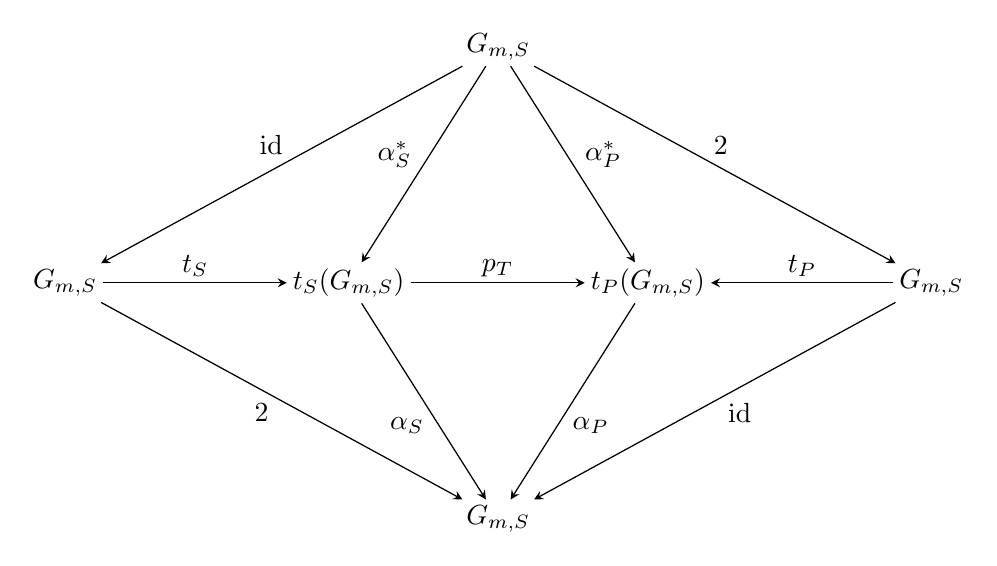
\begin{tikzpicture}[>=stealth,
  every node/.style={inner sep=2pt},
  every path/.style={line width=.45pt}]
  \node (top) at (0,3.0) {$\mathbb G_{m,S}$};
  \node (left) at (-5.5,0) {$\mathbb G_{m,S}$};
  \node (ts) at (-1.9,0) {$t_S(\mathbb G_{m,S})$};
  \node (tp) at (1.9,0) {$t_P(\mathbb G_{m,S})$};
  \node (right) at (5.5,0) {$\mathbb G_{m,S}$};
  \node (bottom) at (0,-3.0) {$\mathbb G_{m,S}$};
  \draw[->] (top) -- node[pos=.48,above left] {$\mathrm{id}$} (left);
  \draw[->] (top) -- node[pos=.55,above left] {$\alpha_S^\ast$} (ts);
  \draw[->] (top) -- node[pos=.55,above right] {$\alpha_P^\ast$} (tp);
  \draw[->] (top) -- node[pos=.48,above right] {$2$} (right);
  \draw[->] (left) -- node[above] {$t_S$} (ts);
  \draw[->] (ts) -- node[above] {$p_T$} (tp);
  \draw[->] (right) -- node[above] {$t_P$} (tp);
  \draw[->] (left) -- node[pos=.48,below left] {$2$} (bottom);
  \draw[->] (ts) -- node[pos=.55,below left] {$\alpha_S$} (bottom);
  \draw[->] (tp) -- node[pos=.55,below right] {$\alpha_P$} (bottom);
  \draw[->] (right) -- node[pos=.48,below right] {$\mathrm{id}$} (bottom);
\end{tikzpicture}
\end{center}
其中间部分就是与典范态射 \(p\circ i\colon\mathrm{SL}_L\to\mathrm P_L\) 相应的 \SGARefLink{sga3:xx:4.1}{4.1} 中的交换图,\footnote{取 \(q=1\).} 该态射诱导上述 \(S\)-初等系之间的态射.

\paragraph{\textbf{5.7.}}
\SGARefTarget{sga3:xx:5.7}
现设 \((G,T,\alpha)\) 是任意 \(S\)-初等系. 考虑交换图
\begin{center}
\begin{tikzpicture}[>=stealth,
  every node/.style={inner sep=2pt},
  every path/.style={line width=.45pt}]
  \node (top) at (0,2.9) {$\mathbb G_{m,S}$};
  \node (left) at (-3.7,0) {$\mathbb G_{m,S}$};
  \node (mid) at (0,0) {$T$};
  \node (right) at (3.7,0) {$\mathbb G_{m,S}$};
  \node (bottom) at (0,-2.9) {$\mathbb G_{m,S}$};
  \draw[->] (top) -- node[pos=.48,above left] {$\mathrm{id}$} (left);
  \draw[->] (top) -- node[left] {$\alpha^\ast$} (mid);
  \draw[->] (top) -- node[pos=.48,above right] {$2$} (right);
  \draw[->] (left) -- node[above] {$\alpha^\ast$} (mid);
  \draw[->] (mid) -- node[above] {$\alpha$} (right);
  \draw[->] (left) -- node[pos=.48,below left] {$2$} (bottom);
  \draw[->] (mid) -- node[left] {$\alpha$} (bottom);
  \draw[->] (right) -- node[pos=.48,below right] {$\mathrm{id}$} (bottom);
\end{tikzpicture}
\end{center}
将此图与 \SGARefLink{sga3:xx:5.6}{5.6} 的图结合, 得到交换图
\begin{center}
\begin{tikzpicture}[>=stealth,
  every node/.style={inner sep=2pt},
  every path/.style={line width=.45pt}]
  \node (top) at (0,2.9) {$\mathbb G_{m,S}$};
  \node (left) at (-4.8,0) {$t_S(\mathbb G_{m,S})$};
  \node (mid) at (0,0) {$T$};
  \node (right) at (4.8,0) {$t_P(\mathbb G_{m,S})$};
  \node (bottom) at (0,-2.9) {$\mathbb G_{m,S}$};
  \draw[->] (top) -- node[pos=.5,above left] {$\alpha_S^\ast$} (left);
  \draw[->] (top) -- node[left] {$\alpha^\ast$} (mid);
  \draw[->] (top) -- node[pos=.5,above right] {$\alpha_P^\ast$} (right);
  \draw[->] (left) -- node[above] {$\alpha^\ast\circ t_S^{-1}$} (mid);
  \draw[->] (mid) -- node[above] {$t_P\circ\alpha$} (right);
  \draw[->] (left) -- node[pos=.5,below left] {$\alpha_S$} (bottom);
  \draw[->] (mid) -- node[left] {$\alpha$} (bottom);
  \draw[->] (right) -- node[pos=.5,below right] {$\alpha_P$} (bottom);
\end{tikzpicture}
\end{center}
利用 \SGARefLink{sga3:xx:4.1}{4.1}, 得到:

\paragraph{\textbf{命题 5.8.}}
\SGARefTarget{sga3:xx:5.8}
\emph{设 \(S\) 是概形, \((G,T,\alpha)\) 是 \(S\)-初等系. 令 \(L=\mathfrak g^\alpha\), 从而 \(L^{-1}=\mathfrak g^{-\alpha}\).}
\emph{\textup{(i)} 存在唯一的群态射 \(f\colon\mathrm{SL}_L\to G\), 满足下列等价条件:}
\[
\begin{array}{ll}
\textup{(a)}
&
f\begin{pmatrix}z&0\\0&z^{-1}\end{pmatrix}=\alpha^\ast(z),
\qquad
f\begin{pmatrix}1&X\\0&1\end{pmatrix}=\exp(X);
\\[1.1em]
\textup{(b)}
&
f\begin{pmatrix}1&X\\0&1\end{pmatrix}=\exp(X),
\qquad
f\begin{pmatrix}1&0\\Y&1\end{pmatrix}=\exp(Y);
\\[1.1em]
\textup{(c)}
&
f\begin{pmatrix}1&X\\0&1\end{pmatrix}=\exp(X),
\qquad
f\begin{pmatrix}0&X\\-X^{-1}&0\end{pmatrix}=w_\alpha(X).
\end{array}
\]
\emph{\textup{(ii)} 存在唯一的群态射 \(g\colon G\to\mathrm P_L\), 满足}
\[
 g(t)=
 \begin{pmatrix}\alpha(t)&0\\0&1\end{pmatrix},
 \qquad
 g(\exp(X))
 =p\begin{pmatrix}1&X\\0&1\end{pmatrix}.
\]
\emph{此外,}
\[
 g(\exp(Y))
 =p\begin{pmatrix}1&0\\Y&1\end{pmatrix},
 \qquad
 g(w_\alpha(X))
 =p\begin{pmatrix}0&X\\-X^{-1}&0\end{pmatrix}.
\]
\emph{态射 \(g\) 忠实平坦且拟紧, 且}
\[
 \Ker(g)=\Ker(\alpha)=\operatorname{Centr}(G),
\]
\emph{而 \(g\circ f\) 是典范态射 \(\mathrm{SL}_L\to\mathrm P_L\).}

注意 \textup{(i)} 中的条件 \textup{(b)} 给出了 \(\mathfrak g^\alpha\) 与 \(\mathfrak g^{-\alpha}\) 之间对偶的显式描述.

\paragraph{\textbf{推论 5.9.}}
\SGARefTarget{sga3:xx:5.9}
\emph{设 \((G,T,\alpha)\) 是 \(S\)-初等系. 则子群}
\[
 T\cdot U_\alpha,\qquad T\cdot U_{-\alpha},
 \qquad U_\alpha,\qquad U_{-\alpha}
\]
\emph{都是闭的.}

由于 \(U_\alpha\) 是 \(T\cdot U_\alpha\) 的闭子群概形, 只须对后者证明此断言. 由 Noether 定理 \textup{(\SGARefLink{sga3:iv:proposition:5:3:1}{第 IV 讲, 5.3.1} 及 \SGARefLink{sga3:iv:lemma:6:4:1}{6.4.1})}, 只须说明
\[
 (T\cdot U_\alpha)/\Ker(\alpha)
\]
是 \(G/\Ker(\alpha)\) 的闭子群. 由 \SGARefLink{sga3:xx:5.8}{5.8}, 这归结为以下显然的事实: \(\mathrm P_L\) 中由 \(c=0\) 定义的子群是闭的; 再次应用 Noether 定理, 也可等价地在 \(\mathrm{GL}_L\) 中处理. 因而\SGARefLink{sga3:xx:1.5}{定理 1.5}\textup{(i)} 中的指数态射是闭浸入.

\smallskip
\noindent\textbf{注意.}\ 此推论也来自 \(T\cdot U_\alpha\) 与 \(T\cdot U_{-\alpha}\) 是 \(G\) 的“Borel 子群”这一事实 \textup{(参见\SGARefLink{sga3:xii:7.10}{第 XII 讲, 7.10})}.

\paragraph{\textbf{5.10.}}
\SGARefTarget{sga3:xx:5.10}
设 \(L\) 是可逆 \(\mathcal O_S\)-模, 且
\[
 \mathbb G_{m,S}\xrightarrow{\ \alpha^\ast\ }T
 \xrightarrow{\ \alpha\ }\mathbb G_{m,S}
\]
是群的图表, 其中 \(T\) 是环面,\footnote{此限定条件由编者补入.} 并且 \(\alpha\circ\alpha^\ast=2\). 设 \(R\) 为 \(\Ker(\alpha)\) 的极大环面, 令 \(K=\alpha^{\ast-1}(R)\). 则 \(K\) 是 \(\mathbb G_{m,S}\) 的乘法型子群; 由于 \(\alpha\circ\alpha^\ast=2\), 它甚至是 \(\mu_{2,S}\) 的子群. 特别地,
\[
 K\longrightarrow\mathrm{SL}_L,
 \qquad
 z\longmapsto\begin{pmatrix}z&0\\0&z^{-1}\end{pmatrix}
\]
在中心内. 因而存在中心群单态射
\[
 K\longrightarrow R\times\mathrm{SL}_L,
 \qquad
 z\longmapsto
 \left(
 \alpha^\ast(z),
 \begin{pmatrix}z&0\\0&z^{-1}\end{pmatrix}
 \right).
\]

设
\[
 G=(R\times\mathrm{SL}_L)/K.
\]
这是 \(S\) 上的仿射光滑群, 纤维连通. 序列
\[
 1\longrightarrow K\longrightarrow
 R\times t_S(\mathbb G_{m,S})
 \xrightarrow{\ u\ }T\longrightarrow1,
 \qquad
 u(x,t_S(z))=x\alpha^\ast(z),
\]
正合. 所以 \(R\times t_S(\mathbb G_{m,S})\) 在 \(G\) 中的像是一个同构于 \(T\) 的环面 \(T'\). 若 \(\alpha'\) 是由 \(\alpha\) 传递到 \(T'\) 上的特征, 则容易检验 \((G,T',\alpha')\) 是 \(S\)-初等系, \(\mathfrak g^{\alpha'}\) 同构于 \(L\), 而 \(\alpha'^\ast\) 由 \(\alpha^\ast\) 通过同构 \(T\xrightarrow{\sim}T'\) 得到. 因而 \SGARefLink{sga3:xx:4.2}{4.2} 中定义的范畴 \(\mathcal D\) 的对象
\[
 \left(
 \mathbb G_{m,S}\xrightarrow{\ \alpha'^\ast\ }T'
 \xrightarrow{\ \alpha'\ }\mathbb G_{m,S},\,
 \mathfrak g^{\alpha'}
 \right)
\]
同构于
\[
 \left(
 \mathbb G_{m,S}\xrightarrow{\ \alpha^\ast\ }T
 \xrightarrow{\ \alpha\ }\mathbb G_{m,S},\,L
 \right).
 \]
由此证明:

\paragraph{\textbf{定理 5.11.}}
\SGARefTarget{sga3:xx:5.11}
\emph{采用 \SGARefLink{sga3:xx:4.2}{4.2} 的记号, 函子}
\[
 (G,T,\alpha)\longmapsto
 \left(
 \mathbb G_{m,S}\xrightarrow{\ \alpha^\ast\ }T
 \xrightarrow{\ \alpha\ }\mathbb G_{m,S},\,
 \mathfrak g^\alpha
 \right)
\]
\emph{是 \(\mathcal E\) 与 \(\mathcal D\) 之间的范畴等价.}

\section{初等系的生成元与关系}
\paragraph{\textbf{6.1.}}
\SGARefTarget{sga3:xx:6.1}
设 \(S\) 是概形, \((G,T,\alpha)\) 是 \(S\)-初等系. 设
\[
 X\in W(\mathfrak g^\alpha)^\times(S),
 \qquad u=\exp(X).
\]
如 \SGARefLink{sga3:xx:3.8}{3.8} 所见, 元素 \(w=w_\alpha(X)\) 特别满足
\[
 (wu)^3=e.
\]
\footnote{编者添加了下面一句.}
以 \(s_\alpha\) 表示 \(\intaut(w)\) 诱导的 \(T\) 的自同构. 由\SGARefLink{sga3:xx:3.1}{定理 3.1}\textup{\SGARefLink{sga3:xx:3.1:item:iii}{(iii)}}, 对每个 \(S'\to S\) 及每个 \(t\in T(S')\), 有
\[
 s_\alpha(t)=\intaut(w)(t)
 =t\,\alpha^\ast\bigl(\alpha(t)^{-1}\bigr).
\]

\paragraph{\textbf{定理 6.2.}}
\SGARefTarget{sga3:xx:6.2}
\emph{设 \(H\) 是 \(S\) 上关于 fppf 拓扑的群层. 设}
\[
 f_T\colon T\longrightarrow H,
 \qquad
 f_\alpha\colon U_\alpha\longrightarrow H
\]
\emph{是群态射, 且 \(h\in H(S)\). 存在 \textup{(必唯一的)} 群态射}
\[
 f\colon G\longrightarrow H
\]
\emph{延拓 \(f_T\) 和 \(f_\alpha\), 并满足 \(f(w)=h\), 当且仅当下列条件成立:}
\emph{\textup{(i)} 对每个 \(S'\to S\)、\(t\in T(S')\) 及 \(x\in U_\alpha(S')\),}
\begin{equation}
\tag{1}\label{sga3:xx:theorem:6-2:equation:1}
 f_T(t)f_\alpha(x)f_T(t)^{-1}
 =f_\alpha(txt^{-1})
 =f_\alpha\bigl(x^{\alpha(t)}\bigr).
\end{equation}
\emph{等价地, \(f_T\) 与 \(f_\alpha\) 可延拓为群态射 \(T\cdot U_\alpha\to H\).}
\emph{\textup{(ii)} 对每个 \(S'\to S\) 及 \(t\in T(S')\),}
\begin{equation}
\tag{2}\label{sga3:xx:theorem:6-2:equation:2}
 h f_T(t)h^{-1}
 =f_T(s_\alpha(t))
 =f_T\!\left(t\,\alpha^\ast(\alpha(t)^{-1})\right).
\end{equation}
\emph{\textup{(iii)} 在 \(H(S)\) 中有以下两个关系:}
\begin{equation}
\tag{3}\label{sga3:xx:theorem:6-2:equation:3}
 h^2=f_T\bigl(\alpha^\ast(-1)\bigr),
\end{equation}
\begin{equation}
\tag{4}\label{sga3:xx:theorem:6-2:equation:4}
 \bigl(hf_\alpha(u)\bigr)^3=e.
\end{equation}

\smallskip
\noindent\emph{证明.}
对 \(U_\alpha\) 和 \(U_{-\alpha}\) 的运算用加法记法, 而其向量空间结构用乘法记法. 若 \(f\) 具有所断言的性质, 则对 \(y\in U_{-\alpha}(S')\), 必有
\[
 f(y)
 =f(w^{-1}wyw^{-1}w)
 =h f_\alpha(w^{-1}yw)h^{-1}.
\]
定义态射 \(f_{-\alpha}\colon U_{-\alpha}\to H\):
\begin{equation}
\tag{\(\ast_1\)}\label{sga3:xx:theorem:6-2:equation:ast-1}
 f_{-\alpha}(y)=h f_\alpha(w^{-1}yw)h^{-1}.
\end{equation}
它是群态射. 在大胞腔 \(\Omega\) 上, 态射 \(f\) 必须满足
\[
 f(ytx)=f_{-\alpha}(y)f_T(t)f_\alpha(x).
\]
这证明了唯一性. 陈述中的条件显然必要; 来证明其充分性.

关系 \textup{\SGARefLink{sga3:xx:theorem:6-2:equation:4}{(4)}} 给出
\[
 h f_\alpha(u)h^{-1}h^2
 =
 f_\alpha(-u)h^{-1}f_\alpha(-u).
\]
由 \textup{\SGARefLink{sga3:xx:theorem:6-2:equation:3}{(3)}} 和 \textup{\SGARefLink{sga3:xx:theorem:6-2:equation:1}{(1)}}, \(h^2=f_T(\alpha^\ast(-1))\) 与 \(f_\alpha(-u)\) 交换, 因而
\[
 h f_\alpha(u)h^{-1}
 =
 f_\alpha(-u)h f_\alpha(-u).
\]
由定义,
\[
 h f_\alpha(u)h^{-1}=f_{-\alpha}(wuw^{-1}),
\]
而 \SGARefLink{sga3:xx:3.7}{3.7} 给出
\begin{equation}
\tag{\(\ast_2\)}\label{sga3:xx:theorem:6-2:equation:ast-2}
 wuw^{-1}=-\widetilde u,
\end{equation}
其中 \(\widetilde u\) 是与 \(u\) 配对的元素. 因此
\begin{equation}
\tag{\(\ast_3\)}\label{sga3:xx:theorem:6-2:equation:ast-3}
 f_{-\alpha}(-\widetilde u)
 =
 f_\alpha(-u)h f_\alpha(-u).
\end{equation}

设 \(t\) 是 \(T\) 在可变的 \(S'\to S\) 上的截面. 对此恒等式施以 \(\intaut(f_T(t))\). 左端得到\footnote{编者更正了下面的计算.}
\[
\begin{aligned}
 f_T(t)f_{-\alpha}(-\widetilde u)f_T(t)^{-1}
 &=
 f_T(t)h f_\alpha(u)h^{-1}f_T(t)^{-1}\\
 &=
 h\bigl(h^{-1}f_T(t)h\bigr)f_\alpha(u)
   \bigl(h^{-1}f_T(t)^{-1}h\bigr)h^{-1}\\
 &=
 h f_T(s_\alpha(t))f_\alpha(u)
   f_T(s_\alpha(t))^{-1}h^{-1}\\
 &=
 h f_\alpha\bigl(\alpha(s_\alpha(t))u\bigr)h^{-1}\\
 &=
 h f_\alpha\bigl(\alpha(t)^{-1}u\bigr)h^{-1}\\
 &=
 f_{-\alpha}\bigl(-\alpha(t)^{-1}\widetilde u\bigr).
\end{aligned}
\]
这里用了 \textup{\SGARefLink{sga3:xx:theorem:6-2:equation:2}{(2)}}, \textup{\SGARefLink{sga3:xx:theorem:6-2:equation:1}{(1)}}, \(s_\alpha(t)=t\alpha^\ast(\alpha(t)^{-1})\) 及 \(\alpha\circ\alpha^\ast=2\).

\((\ast_3)\) 的右端经共轭后成为
\[
 f_\alpha(-\alpha(t)u)\,
 f_T(t)h f_T(t)^{-1}h^{-1}\,
 h f_\alpha(-\alpha(t)u).
\]
由于
\[
 h f_T(t)^{-1}h^{-1}
 =f_T(s_\alpha(t^{-1}))
  =f_T\bigl(t^{-1}\,\alpha^\ast(\alpha(t))\bigr),
\]
它等于
\[
 f_\alpha(-\alpha(t)u)\,
 f_T\bigl(\alpha^\ast(\alpha(t))\bigr)\,
 h f_\alpha(-\alpha(t)u).
\]
比较得
\[
 f_{-\alpha}\bigl(-\alpha(t)^{-1}\widetilde u\bigr)
 =
 f_\alpha(-\alpha(t)u)\,
 f_T\bigl(\alpha^\ast(\alpha(t))\bigr)\,
 h f_\alpha(-\alpha(t)u).
\]
由于 \(\alpha\colon T\to\mathbb G_{m,S}\) 忠实平坦, 且 \(H\) 是分离预层, 可以把 \(-\alpha(t)^{-1}\) 换成 \(\mathbb G_{m,S}\) 的任意截面. 因此:

\paragraph{\textbf{引理 6.2.1.}}
\SGARefTarget{sga3:xx:6.2.1}
\emph{对每个 \(S'\to S\) 及每个 \(z\in\mathbb G_m(S')\),}
\[
 f_{-\alpha}(z\widetilde u)
 =
 f_\alpha(z^{-1}u)\,
 f_T\bigl(\alpha^\ast(-z^{-1})\bigr)\,
 h f_\alpha(z^{-1}u).
\]

设 \(x,y\in\mathbb G_a(S')\), 其中 \(S'\to S\), 并假设 \(y\) 和 \(1+xy\) 可逆. 首先对 \(z=y\) 应用\SGARefLink{sga3:xx:6.2.1}{引理 6.2.1}, 得到\footnote{编者展开了以下计算.}
\[
 f_\alpha(xu)f_{-\alpha}(y\widetilde u)
 =
 f_\alpha\bigl((x+y^{-1})u\bigr)\,
 f_T\bigl(\alpha^\ast(-y^{-1})\bigr)\,
 h f_\alpha(y^{-1}u).
\]
现在 \(x+y^{-1}=y^{-1}(1+xy)\). 对 \(z=y/(1+xy)\) 应用引理, 得
\[
\begin{aligned}
 f_\alpha\bigl((x+y^{-1})u\bigr)
 &=
 f_{-\alpha}\!\left(\frac{y}{1+xy}\widetilde u\right)
 f_\alpha\bigl(-(x+y^{-1})u\bigr)\\
 &\qquad{}\cdot h\,
 f_T\!\left(\alpha^\ast\!\left(-\frac{y}{1+xy}\right)\right).
\end{aligned}
\]
代入前一恒等式, 得
\[
\begin{aligned}
 f_\alpha(xu)f_{-\alpha}(y\widetilde u)
 &=
 f_{-\alpha}\!\left(\frac{y}{1+xy}\widetilde u\right)
 f_\alpha\bigl(-(x+y^{-1})u\bigr)h^{-1}\\
 &\qquad{}\cdot
 f_T\bigl(\alpha^\ast(1+xy)^{-1}\bigr)
 h f_\alpha(y^{-1}u).
\end{aligned}
\]
由 \textup{(2)}, \(h^{-1}f_T(t)h=f_T(s_\alpha(t))\) \textup{(回顾 \(s_\alpha^2=\operatorname{id}\))}, 且 \(s_\alpha\circ\alpha^\ast=-\alpha^\ast\), 因而上式为
\[
\begin{aligned}
 f_{-\alpha}\!\left(\frac{y}{1+xy}\widetilde u\right)
 f_\alpha\bigl(-(x+y^{-1})u\bigr)
 f_T\bigl(\alpha^\ast(1+xy)\bigr)
 f_\alpha(y^{-1}u).
\end{aligned}
\]
对 \(x'\in U_\alpha(S')\) 和 \(z\in\mathbb G_m(S')\), 有
\[
 f_\alpha(x')f_T(\alpha^\ast(z))
 =
 f_T(\alpha^\ast(z))f_\alpha(z^{-2}x').
\]
所以
\[
\begin{aligned}
 f_\alpha(xu)f_{-\alpha}(y\widetilde u)
 &=
 f_{-\alpha}\!\left(\frac{y}{1+xy}\widetilde u\right)
 f_T\bigl(\alpha^\ast(1+xy)\bigr)\\
 &\qquad{}\cdot
 f_\alpha\!\left(
 \left[
 -\frac{y^{-1}(1+xy)}{(1+xy)^2}+y^{-1}
 \right]u
 \right)\\
 &=
 f_{-\alpha}\!\left(\frac{y}{1+xy}\widetilde u\right)
 f_T\bigl(\alpha^\ast(1+xy)\bigr)
 f_\alpha\!\left(\frac{x}{1+xy}u\right).
\end{aligned}
\]
由此证明:

\paragraph{\textbf{引理 6.2.2.}}
\SGARefTarget{sga3:xx:6.2.2}
\emph{设 \(S'\to S\). 若 \(a\in U_\alpha(S')\)、\(b\in U_{-\alpha}^\times(S')\), 且 \(1+ab\in\mathbb G_m(S')\), 则}
\[
 f_\alpha(a)f_{-\alpha}(b)
 =
 f_{-\alpha}\!\left(\frac{b}{1+ab}\right)
 f_T\bigl(\alpha^\ast(1+ab)\bigr)
 f_\alpha\!\left(\frac{a}{1+ab}\right).
\]

由概形稠密性, 对满足 \(1+ab\) 可逆的 \(b\in U_{-\alpha}(S')\), 此公式仍成立. 定义
\[
 f\colon\Omega\longrightarrow H,
 \qquad
 f(ytx)=f_{-\alpha}(y)f_T(t)f_\alpha(x).
\]
由\SGARefLink{sga3:xx:6.2.2}{引理 6.2.2}、条件 \SGARefLink{sga3:xx:6.2}{6.2}\textup{(i)} 以及 \SGARefLink{sga3:xx:2.4}{2.4} 的公式 \textup{(F')}, 立即可知只要 \(g,g'\in\Omega(S')\) 且 \(gg'\in\Omega(S')\), 就有
\[
 f(gg')=f(g)f(g').
\]
因此, 由\SGARefLink{sga3:xviii:prop:2.3}{第 XVIII 讲, 2.3}\textup{\SGARefLink{sga3:xviii:prop:2.3:item:iii}{(iii)}} 及 \SGARefLink{sga3:xx:2.4}{2.4},\footnote{例如由 \SGARefLink{sga3:xx:section:1}{1.1}, \(G\) 的每个几何纤维都连通.} 存在延拓 \(f\) 的群态射 \(G\to H\), 仍记为 \(f\). 还只须证明 \(f(w_\alpha)=h\). 由于
\[
 w_\alpha=u\cdot(-\widetilde u)\cdot u,
\]
公式 \((\ast_3)\) 给出\footnote{编者通过引用 \((\ast_3)\) 简化了原来的论证.}
\[
 f(w_\alpha)
 =f_\alpha(u)f_{-\alpha}(-\widetilde u)f_\alpha(u)
 =h.
\]
\SGARefLink{sga3:xx:6.2}{定理 6.2} 证明完成.

\paragraph{\textbf{注 6.3.}}
\SGARefTarget{sga3:xx:6.3}
\emph{这些结果将在\SGARefLink{sga3:xxiii:subsection:3-5}{第 XXIII 讲, 3.5} 中补全.}
